%----- Author : Kang Yen -----%
%----- Version: 1.0        -----%
%----- Date   : 2019.06    -----%

\documentclass[12pt]{ksthesis}
\usepackage[cmex10]{amsmath}
\usepackage{amsthm}
\usepackage{latexsym}
\usepackage{./class/psfig}
\usepackage{./class/fancyheadings}
\usepackage{./class/citesort}
\usepackage{graphicx}
\usepackage{subfigure}
\usepackage{amssymb}
\usepackage{algorithm}
\usepackage{algorithmic}
\usepackage{multirow}
\usepackage{cite}

\newtheorem{thm}{Theorem}
\newtheorem{lemma}{Lemma}
\newtheorem{defi}{Definition}
\newtheorem{proposition}{Proposition}
\newtheorem{cor}{Corollary}

\paperwidth=21cm \paperheight=29.7cm

\doublespace

\title{National Cheng Kung University
     \\Institute of Computer and Communication Engineering
     \\Master Thesis}
\author{}

\phdthesis

\Thesisspace

\begin{document}

\begin{preliminary}
%---------- Preliminary ----------%
\setcounter{page}{2} \large


\begin{abstract}
%------------------------- Abstract -------------------------%
\begin{center}

{\Large Implementation of Vehicle Dispatching and Monitoring in a Self-Driving Delivery Emulation System for Urban Areas\vspace{0.4cm}}

\end{center}

\begin{center}

{\large Kang Yen\vspace{0.2cm} \\ Institute of Computer and
Communication Engineering \vspace{0.2cm}\\ National Cheng Kung
University \\ }

\end{center}

\Thesisspace {\large 
Freight transportation plays an important role in daily life. As the e-commence and traffic technology developed, customers have high expectations for the more rapid and more flexible parcel delivery service. However, due to rising labor costs, the delivery mode of autonomous cars is one of alternatives. By reviewing the self-driving technology, the maturity of technology and profitable business model are the concerns. Moreover, so far there is no complete self-driving delivery system in Asia.
 
As a result, the paper integrated traffic simulation software SUMO and mobile application to simulate the package delivery service. Moreover, this study proposed a vehicle dispatching and monitoring system, which can cope with delivery orders, arrange routes, monitor vehicle’s movements, and demonstrate loading and unloading details of trucks. At the same time, this paper proposed dynamic dispatching mechanism consisting of box filtering stage and simple time scheduling stage. The mechanism can judge whether the delivery order could be established. Finally, the paper ran the parcel delivery simulation in the downtown area of Tainan, which showed clear visualization of logistic condition in the simulation results.

Using this proposed system has three advantages. One is that the user can experience more immediate and more flexible delivery service. Second is that administrator can monitor the vehicle’s route and the vehicle’s real-time behavior. Third is that the developer can extend more complex routing algorithm, and add new application on the simulation platform.
}

\emph{\textbf{Keywords}}---self-driving delivery, traffic simulation, dynamic dispatching mechanism, package delivery service.

\end{abstract}

\begin{acknowledgements}
%------------------------- Acknowledgement -------------------------%
\Thesisspace {\large First of all, I would like to express my gratitude to my advisor, Professor Kuo-Feng Ssu, for his valuable advices in my research and encouragement during my time at National Cheng Kung University. I am exceptionally thankful for his endless effort to provide guidance of paper reading and thesis writing.

Besides, I am really grateful to Professors Hewijin Christine Jiau for not only her contributions to the research but also serving on my dissertation committee.
I am obliged to the members of Dependable Computing Laboratory, including Yu-Jung Change, Che-Ming Lee, Wei-Lun Hung, Wen-Chin Lai, and Chun-Ting Po. They helped me a lot and gave me many opinions in my research.
Finally, I would like to thank my family and friends for their support.}

\end{acknowledgements}

\tableofcontents \listoffigures\clearpage

\end{preliminary}
%---------- Preliminary ----------%
\begin{thesis}\large {
%------------------------- Introduction -------------------------%
\chapter{Introduction} \label{Chap:Introduction}

Freight transportation problem is an important issue in our daily lives \cite{Anand2012} . With the development of transportation technology, the customers have the higher expectation on more efficient and more rapid delivery service. Besides, as the self-driving car technology grows \cite{Lutin2013}, the self-driving vehicle delivery begins to be a crucial research topic. After reviewing the self-driving car delivery market, there is no complete self-driving delivery system. 
Before introducing the autonomous cars to the real road network, so far the thesis wants to focus on building the software part of the whole system, which can run package delivery simulation. As the software part of the system can be established, the administrator can get the car’s real-time information including vehicle’s location, the container’s values, and the vehicle’s speed. As a result, in the future the user can apply the above functions into the actual self-driving cars for achieving the goal of system integration directly.

As illustrated in Figure 1.1, this thesis implemented a vehicle dispatching and monitoring system in the red frame. This system includes two main components such as Simulation of Urban Mobility (SUMO) simulator and a SUMO server. The SUMO server was implemented by Traffic Control Interface, which have the access to retrieve the vehicle’s values or manipulate the vehicle’s behaviors on a running road traffic simulation.

\begin{figure}[t!]
\centering
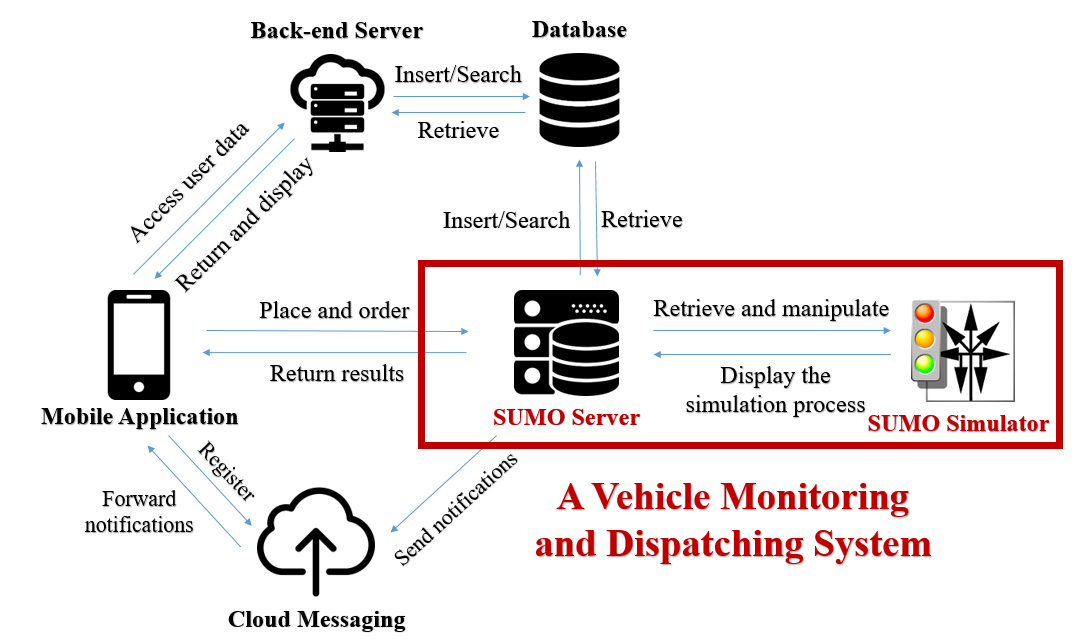
\includegraphics[width=0.85\textwidth]{./Thesis_figures/F1-1_System_Design_Overview.PNG}

\caption{\large A Vehicle dispatching and monitoring system.}
\vspace{0.5cm}
\label{Fig:System_Overview}
\end{figure}

In the previous scheme \cite{Jiang2018}, senders can select their delivery time, but receivers only can wait for the coming parcels passively. This delivery service has the problem that the arrival time of parcels does not match receivers’ available time, which leads to the loss of taking delivery of goods. Hence, the thesis offers a new delivery service where receivers have the chances to select their expected arrival time of the package, which can improve the delivery loss problem. This thesis illustrates the flow chart of the new delivery process including the sender’s part and the receiver’s part.

Besides, the SUMO server develops a dispatching mechanism to deal with the order requests, and arranges the routes dynamically and immediately. In this mechanism, vehicles have to pass through the two stages. First is box filtering stage, which filters out the vehicle without the available space of the appointed box size, and the other vehicles can enter into the second stage named as simple time scheduling stage. This stage would judge whether the order can be inserted into the original time schedule or nor. Moreover, the thesis would demonstrate that the dispatching mechanism would be applied to the scenario of the sender and the receiver in the different ways.

Finally, the thesis installs the SUMO simulator, cleans up the map of the downtown area of Tainan, sets up the parameters, and ran the simulation with five scenarios of the delivery service.

To sum up, the thesis is organized as follows. Chapter 1 describes the motivation of research and the background of self-driving delivery and the purpose of building the system. Chapter 2 presents the related work. The whole system design overview is proposed in Chapter 3. The implementation of a vehicle dispatching and monitoring system is described in Chapter 4. Chapter 5 shows flow charts of the delivery process.  Chapter 6 illustrates how the dispatching mechanism works. The simulation result is presented in Chapter7. Finally, conclusion and future work are discussed in Chapter 8.


  


\chapter{Related Work} \label{Chap:Related}
%------------------------- Related Works -------------------------%

\section{Home Delivery}
As the e-commence and the technology of logistics has developed for several years, this bought about the general tendency in logistics toward higher delivery frequency, single orders, and smaller freight \cite{Visser2014}.


In the freight transportation industry, logistics models can be divided into several types of logistic channel including post, shelf picking, dedicated warehouse, workspace, and home delivery.

Gevaers et al. developed a cost simulation tool, which showed that the Last Mile delivery is one of the most expensive stages of the entire e-logistics chain \cite{Gevaers2014}. Besides, in the Last Mile delivery, the most widespread delivery mode is home delivery.

As the result, home delivery (HD) is a crucial topic to discuss, retailers delivered a large amount of the daily consignment to the customer’s home. So far home delivery can be a delivery point to one’s home address, to another address, or to a pickup point  \cite{Zhou2016}. 

However, there are some issues about home delivery, including delay of delivery service, the customer’s absence at home, and too long delivery time. Thus, to meet the increasing demand of more rapid parcel delivery service, a small aerial vehicle is proposed by the professors in George Mason University \cite{Ali2015}.

A multi-rotor aerial vehicle can provide the fast and urgent parcel delivery service such as rapid food delivery and remote medical supply delivery. However, this application has some design technical difficulties, which includes extending battery life, handling the increasing weight of the parcel, and dealing with the sudden climate change \cite{Ali2015}. In one word, an aerial vehicle has lower reliability, scalability and capacity than a delivery truck.

Moreover, \cite{Sawadsitang2018} introduced a joint ground and aerial delivery service framework. The framework consists of two delivery modes, which can complement each other due to their unique features and benefits. With this integration of ground-based delivery and drone delivery, the approach not only can cope with sudden service interruption like accident, but also can maximize service quality and minimize cost. However, this approach has the problem of the uncertainty in customer’s demand and computation time of routing the delivery path. 

%% [9], [10]
In some metropolitan areas in the U.S. like Seattle, \cite{Sheth2019} deployed alternative delivery mode such as cargo bikes. Due to the increasing freight volumes on the road and scarce road space, cargo bicycles are being utilized for the last mile deliveries in several urban cities \cite{Melo2017}. The advantage of using delivery bikes is that cargo bicycles are not encumbered by the same parking and congestion constraints as trucks. However, the disadvantage is that cargo bikes are less cost effective for greater distances than delivery trucks.

%% [11]
In China, \cite{Delivery2017} showed that JD.com, which is the largest e-commence platform by revenue, used autonomous driving vehicles to hit the open road in Beijing. The vehicle can store up to thirty containers, and can travel 15 km/hr. The current concerns of this approach are the autonomous driving technology and government regulations.

\section{Traffic Simulation}
SUMO is an open source traffic simulation package including net import and demand modeling components. Besides, SUMO helps to investigate several research topics, which includes route choice and simulating vehicular communication  \cite{Krajzewicz2007}.

%% [13]
\cite{10.1007/978-3-662-45079-6_5} introduced the real-time I/O data interface and proposed an approach to building up a Web service. Beside, by knowing the commands of traffic control interface (TraCI), the user can handle the communication with SUMO Traffic Simulation Suite. Finally, \cite{10.1007/978-3-662-45079-6_5} demonstrated an example of the code, which provides the base for a new Web service called TraaS (TraCI as a service).

%% [14]
\cite{Tunku2016} showed the transportation simulation for food distribution. The author used TraaS to assign trucks backup when the original tricks unable to cover the destination shops at certain time threshold, and re-route the path for the backup vehicles.

%% [15]
\cite{Kendziorra2015} aims to achieve simulation scenarios in which incidents occur, and introduced the implementation of logistic transport. The concept of freight and goods was implemented to enable the simulation of good traffic, which consists of the containers and stop.



\chapter{System Design Overview}\label{Chap:Architecture}
%-------- System Architecture--------%

\section{A Whole System}

\begin{figure}[t!]
\centering
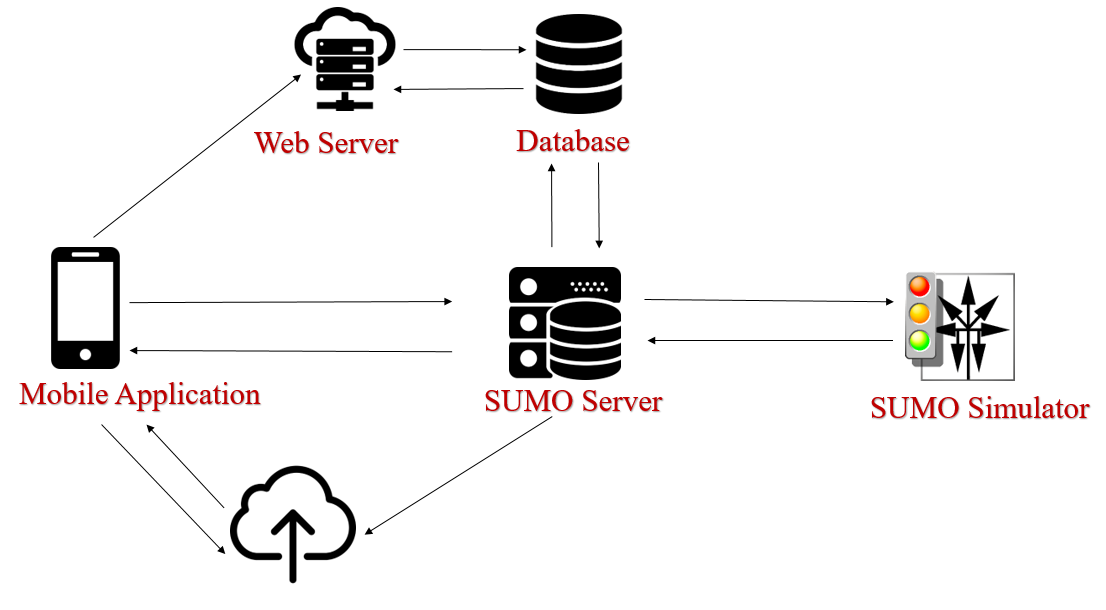
\includegraphics[width=0.85\textwidth]{./Thesis_figures/F3-1_a_whole_system.PNG}
\caption{\large A Whole System.}
\vspace{0.5cm}
\label{Fig:A_Whole_System}
\end{figure}

The chapter aims to design a vehicle dispatching and monitoring system that can deal with the parcel delivery order request from the mobile application. In addition, the system can dispatch the vehicle to the destination, visualize the route of vehicles, and retrieve the information of the vehicle in SUMO simulator.
As illustrated in Figure 3.1, the whole system consists of four main components, including a SUMO server, a SUMO simulator, the mobile application, and a web server with database.

\subsection{SUMO Server}
A SUMO server initializes the road traffic condition including the map, traffic lights, and the moving vehicles with package delivery missions. Besides, the SUMO server communicates with a SUMO simulator via a specific port address.

\subsection{SUMO Simulator}
After receiving the commands from the SUMO server, a SUMO simulator would execute the action of commands in SUMO-GUI,  or change the state of the simulated objects.

\subsection{Mobile Application}
The mobile application is responsible for shipping a delivery order request to SUMO server. After computation of the server and the simulator, the mobile application would obtain the computed feedback from the SUMO server.

\subsection{Web Server with Database}
If the delivery order is generated successfully after dispatching computation of SUMO server, the data of the delivery order from the server side would be inserted into the database. Furthermore, the mobile application can trace the logistic information when retrieving the information of delivery order from the web server.

\section{A Vehicle Dispatching and Monitoring System}
As illustrated in Figure 1.1, a vehicle dispatching and monitoring system has two components, including a SUMO simulator and a SUMO server.



\subsection{SUMO Simulator}
A SUMO simulator has two jobs. One is to receive the commands from SUMO server. The commands include retrieving the values of simulated objects and manipulating online behavior in SUMO-GUI. Second is to return the retrieval messages such as the current road id of the specific vehicle. Besides, the simulator could display the visualization of the vehicle’s movement, and show the change of the vehicle’s state in SUMO-GUI.

\subsection{SUMO Server}
A SUMO server has three main jobs. One is to communicate with the Android client and the database. Second job is to compute the routing arrangement. Third job is to send commands to control the behavior of the simulated objects in the running simulation.

\chapter{Implementation of Vehicle Dispatching and Monitoring System }\label{Chap:Architecture}
%---------- Implementation -------------------%

To build a vehicle dispatching and monitoring system, the thesis has to implement two components, which includes SUMO simulator and SUMO server. According to the concept of web service in [13], the thesis improved the architecture of web service to meet the demands of Android client.
As illustrated in Figure 4.1, this architecture involves three parts, including SUMO simulator, Real-time I/O data Interface and Android Client.

\begin{figure}[t!]
\centering
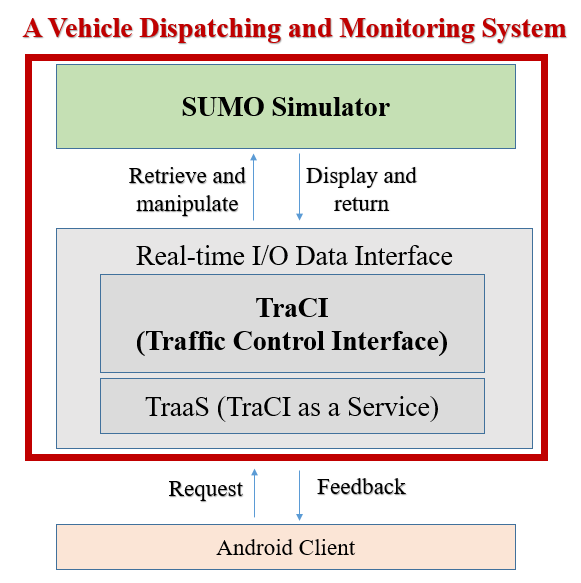
\includegraphics[width=0.85\textwidth]{./Thesis_figures/F4-1_webService_arcitecture.PNG}
\caption{\large Improved architecture of web service.}
\vspace{0.5cm}
\label{Fig:Improved_architecture_of_web_service}
\end{figure}



\section{Traffic Control Interface}
To interact with a simulation, Real-time I/O data Interface offers a possibility to communicate between the simulation and the user application bi-directionally \cite{Fischer}. Besides, Traffic Control Interface, which is called “TraCI”, is a kind of Real-time I/O data Interface in SUMO suite.
TraCI can implement online interaction with the simulation ,and have the access to a running road traffic simulation. This access allows TraCI to retrieve values of simulated objects, and to manipulate their online behavior.
To consider the portability of system implementation and the popularity in web service, this study selects TraaS as the traffic control interface. TraaS is a java library for working with TraCI, which is viewed as a java traci client. The client can be used to write TraCI scripts directly, and TraaS stands for TraCI as a Service.

\subsection{TraCI to SUMO Simulator}
Before communicating with the SUMO simulator, TraCI would establish a connection to SUMO. As illustrated in Figure 4.2, TraCI client connects to SUMO by setting up a TCP connection to the to the appointed SUMO port. As a result, SUMO can interact with TraCI client, and SUMO receives commands from the client application, which have the influence on a vehicle’s behavior and environment details.

\begin{figure}[t!]
\centering
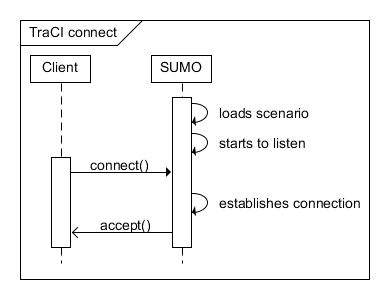
\includegraphics[width=0.85\textwidth]{./Thesis_figures/F4-2_TraCI_connection.PNG}
\caption{\large The connection of Traffic Control Interface.}
\vspace{0.5cm}
\label{Fig:TraCI_connection}
\end{figure}


\subsection{TraCI to Android Client}
Before communicating with the Android client, TraaS would create a thread, which acts a socket server. This server has an appointed port to connect to Android client. When the system runs the main program of TraaS, the thread of socket server would run synchronically. As a result, TraaS can receive the request from Android client and output the computation feedback to Android via the socket server channel.

\section{Manipulation of Vehicle Routing}
When it comes to value retrieval in SUMO, there are fifteen data types in TraCI commands. The most important data type is vehicle value retrieval. For instance, when TraaS executes the command of getRoadID, the SUMO simulator would return the id of the edge which the named vehicle was at.

\textbf{getRoadID (String vehID) $\rightarrow$ return String edgeID}


Another example of vehicle value retrieval is setRoute, which could change the named vehicle’s route to given edges list.

\textbf{setRoute(String vehID, list edgeList)$\rightarrow$ return None}

serRoute(“1”, [“2”, ”4”, ”6”]) this changes route for the vehicle ID 1 to edges 2-4-6

Besides, TraaS manipulates the simulated objects like vehicles via state changing commands. For example, when TraaS executes setStop function, the simulator would add a stop at the given edge and lane, and the vehicle will stop for the given duration or end stopping at the given until attribute.
 
\textbf{setStop (String vehID, String edgeID, double pos, byte laneIndex, double duration, SumoStopFlags sf, double startPos, double until) $\rightarrow$ return None}
 
The following two figures show how the SUMO simulator manipulates the vehicle’s behavior after executing the commands of changing route and setting stop.
As illustrated in Figure 4.3, when the simulation time is 1472 seconds, the vehicle 2 occurrs at the left lower corner, and the yellow path is the vehicle 2’s route. 
The end edge id of the vehicle 2 is located at Chung Cheng Gym in National Cheng Kung University.

\begin{figure}[t!]
\centering
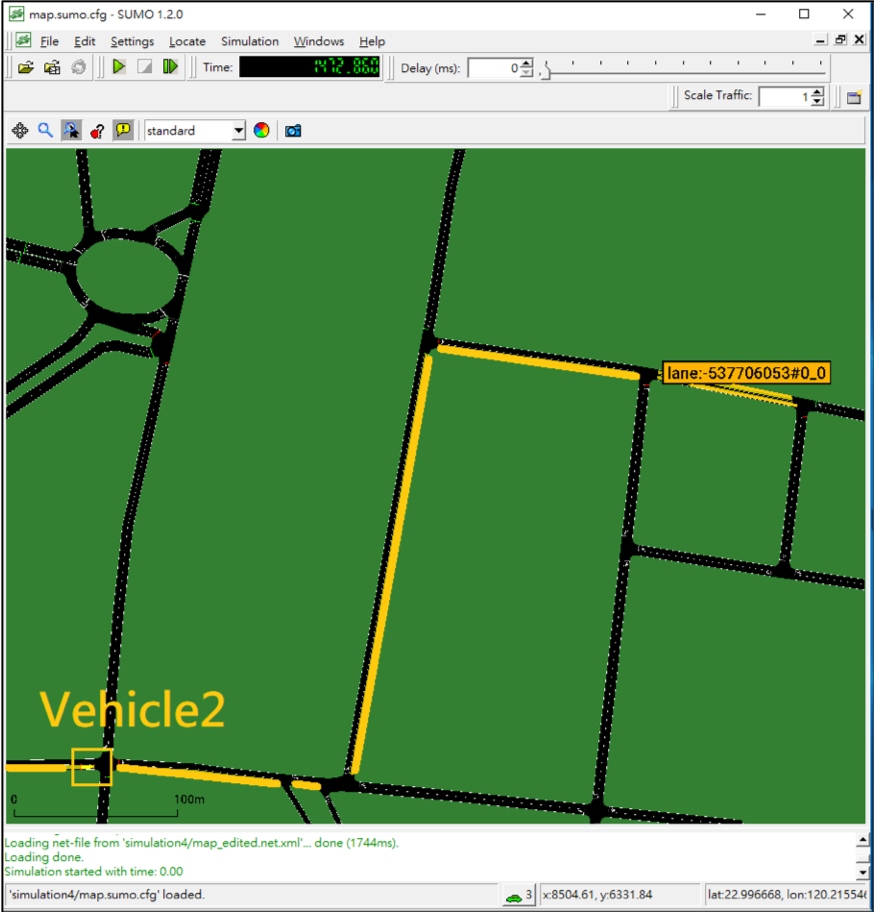
\includegraphics[width=0.85\textwidth]{./Thesis_figures/F4-3_Change_endEdge.PNG}
\caption{\large Change the end edge of the destination.}
\vspace{0.5cm}
\label{Fig:Change_endEdge}
\end{figure}

\begin{figure}[H]
\centering
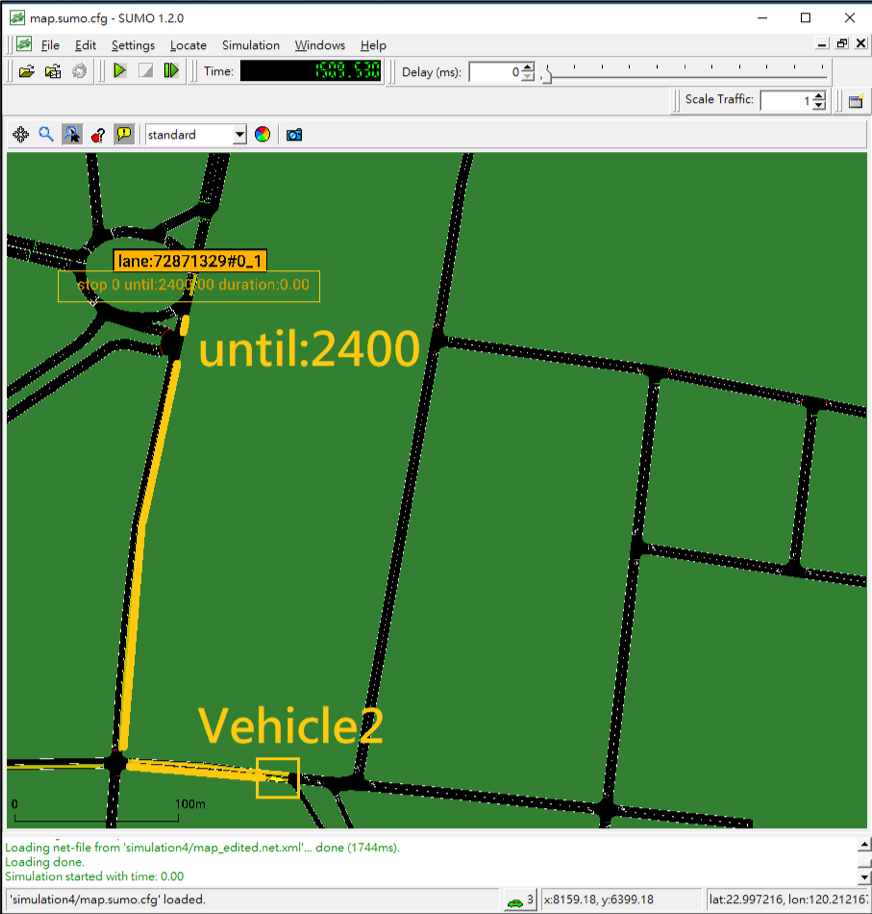
\includegraphics[width=0.85\textwidth]{./Thesis_figures/F4-4_setStop.PNG}
\caption{\large Set stop at the destination.}
\vspace{0.5cm}
\label{Fig:Set_stop}
\end{figure}


As illustrated in Figure 4.4, at the 1500 simulation seconds, the vehicle 2 cancels the previous route whose end edge id was \textbf{“-537706053\#0”}, and the simulator replaces the original route of vehicle 2 in Figure 4.3 with a new route. The end edge id of this new route is \textbf{“72871329\#0”}, which is at Tainan Train Station. Furthermore, the vehicle 2 would stop at the edge \textbf{“72871329\#0”}, and would stay in the same position until 2400 simulation seconds.



\section{Map Address Conversion}

\begin{figure}[H]
\centering
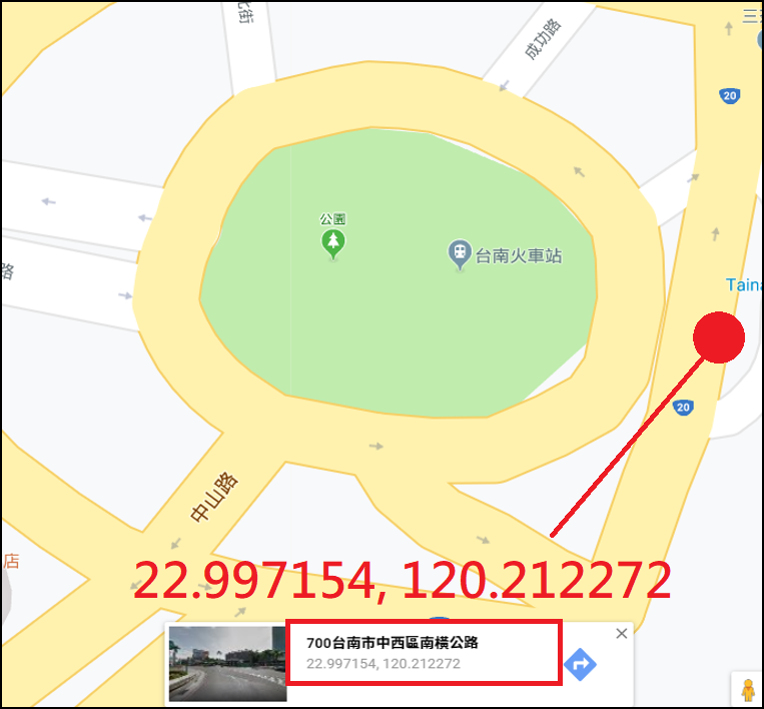
\includegraphics[width=0.85\textwidth]{./Thesis_figures/F4-5_GPS_googleMap.PNG}
\caption{\large The latitude and longitude in Google Map.}
\vspace{0.5cm}
\label{Fig:GPS_in_GoggleMap}
\end{figure}


When the user submits the delivery order request in the mobile application, the app would parse the sender address into the latitude and longitude of a point using Google Map API (Application Programming Interface).
As illustrated in Figure 4.5, when the user inputs the address of Tainan Train Station, Google Map would show the red pinpoint of the address, and display the latitude and longitude (22.997154, 120.212272).

Furthermore, TraaS converts the longitude and latitude to roadID, laneIndex, and pos. RoadID identifies a road segment (edge), and pos describes the position of the node in longitudinal direction (ranging from 0 to the road's length). Finally, laneIndex identifies the driving lane on the road segment.
As illustrated in Figure 4.6, TraaS converts the latitude and longitude of Tainan Train Station into the roadID (“72871329”), pos (5.6), and laneIndex (0).
TraaS uses the sender’s edge of to arrange the vehicle’s route and sets stopping address in the SUMO simulator according to the section 4.2.

\begin{figure}[H]
\centering
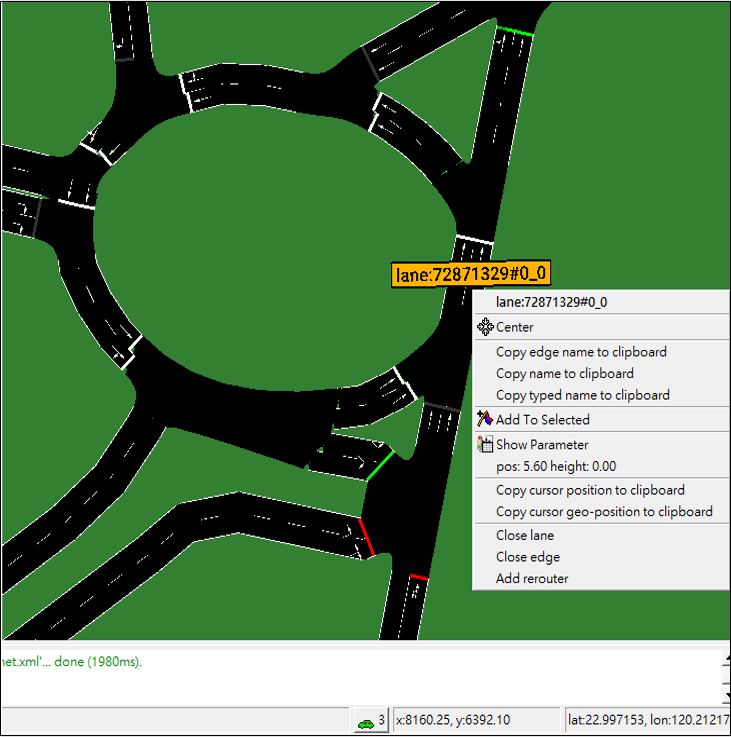
\includegraphics[width=0.85\textwidth]{./Thesis_figures/F4-6_GPS_SUMOMap.PNG}
\caption{\large Convert the latitude and longitude into a road segment and pos.}
\vspace{0.5cm}
\label{Fig:Convert_To_Road}
\end{figure}




\chapter{Flow Chart of Parcel Delivery Process}\label{Chap:Flow Chart of Parcel Delivery Process}

The chapter aims to illustrate the flow chart of parcel delivery process, containing the sender’s scenario and the receiver’s scenario.

\section{Sender Part}

\begin{figure}[H]
\centering
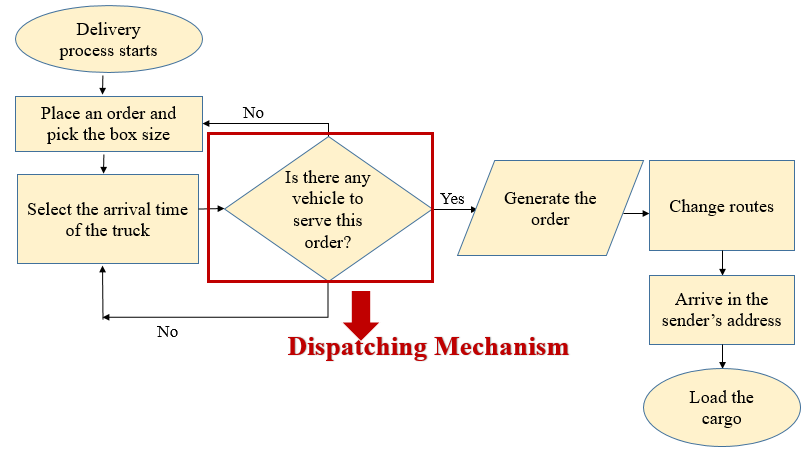
\includegraphics[width=1.14\textwidth]{./Thesis_figures/F5-1_sender_delivery_process.PNG}
\caption{\large The sender’s parcel delivery process.}
\vspace{0.5cm}
\label{Fig:sender_process}
\end{figure}

Figure 5.1 evaluates the sender’s parcel delivery process.


\begin{itemize}
\item
The parcel delivery process starts at 09:00 AM.

\item
The user places a delivery order, which includes the sender’s address, the receiver’s id, the receiver’s appointed address. Then,the user picks the box size categorized into small size, medium size, and large size.


\item
The user selects the sender’s arrival time interval of the parcel, and the selection of arrival time starts from 09:30 AM to 03:00 PM with the interval of thirty minutes. Then, the mobile application forwards the order request to the SUMO server.

\item
After receiving the order request, the SUMO server would use dispatching mechanism to judge whether the system have available vehicles to serve this request. If there is no vehicle meeting the demand, the user would receive the failure feedback of the request. Thus, the user would be asked to pick the arrival time again, or change the box size, and submit the edited request once more.
In contrast, if there is an available vehicle which can serve this delivery order, the order would be generated by the database successfully.

\item
When the delivery order is established, the unique index number of the box would be generated for binding to this sender’s order.

\item
Therefore, the SUMO server dispatches the vehicle to the sender’s appointed address, and the vehicle would park at the address.

\item
When the vehicle arrives to the sender’s appointed address, the sender would get the notification on the mobile application, and begin to load the delivery package into the truck.

\item
When the truck finishes the loading task, the system would end this sender’s delivery process.

\end{itemize}

\section{Receiver Part}

\begin{figure}[H]
\centering
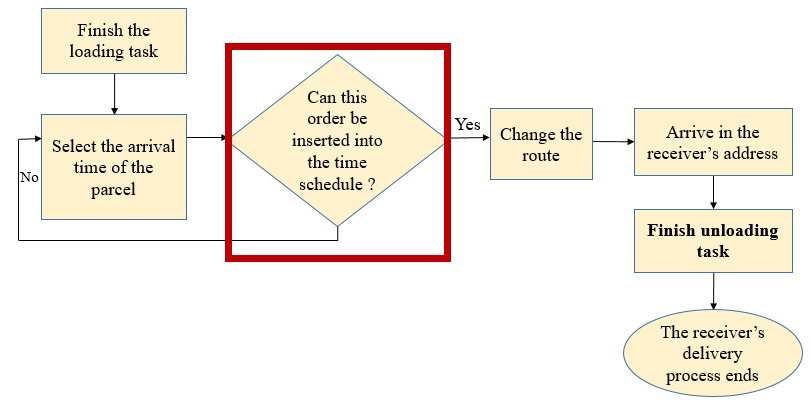
\includegraphics[width=1.14\textwidth]{./Thesis_figures/F5-2_receiver_delivery_process.PNG}
\caption{\large The receiver's parcel delivery process.}
\vspace{0.5cm}
\label{Fig:receiver_process}
\end{figure}

Figure 5.2 evaluates the receiver’s parcel delivery process

\begin{itemize}
\item
As the vehicle finishes the loading task at the sender’s appointed address, the SUMO server will use FCM to forward the notification to the receiver.

\item
After getting the notification of completing loading task, the logistic status would change. As a result, the receiver can go to “my received parcel” page and select the receiver’s arrival time of the parcel. This parcel consists of many details such as the vehicle id, the box index number, sender’s id, the content of parcel, and the order number. Besides, the selection of arrival time begins at 09:30 AM to 03:00 PM with the interval of half an hour.

\item
Then, the SUMO server would check whether the receiver’s delivery order can be established or not. If this request of the order fails, the receiver can select another suitable arrival time again. On the other hand, if the request of the receiver’s order can be accepted by the parcel delivery schedule, the receiver will be informed the order is established successfully.

\item
When the delivery schedule changes due to the new order insertion, the SUMO server will set new routes on the dispatched vehicle.

\item
As the vehicle arrives to the receiver’s appointed address, the receiver would receive the arriving notification.

\item
After the vehicle unloads the parcel successfully, the receiver’s delivery process would end.

\end{itemize}


\chapter{Dispatching Mechanism}\label{Chap:Dispatching Mechanism}
The chapter aims to how the system uses dispatch mechanism to judge whether the sender’s delivery order can be established.
As illustrated in Figure 6.1, the dispatching mechanism consists of two filtering stages. One is box filtering stage, and the second is simple time scheduling stage. After the user places the delivery order, picks the box size, and selects the arrival time of the parcel, the order request would enter into the box filtering stage.
If all vehicles do not have any space for this picked box size, the user would select the other choice of box size. In contrast, if the vehicle’s box capacity is lower than three, this vehicle is qualified to enter into second filtering stage (simple time scheduling stage) 
Furthermore, if there are no available vehicles that can serve this order in the simple time scheduling stage, the user should pick the other appropriate arrival time.

\begin{figure}[H]
\centering
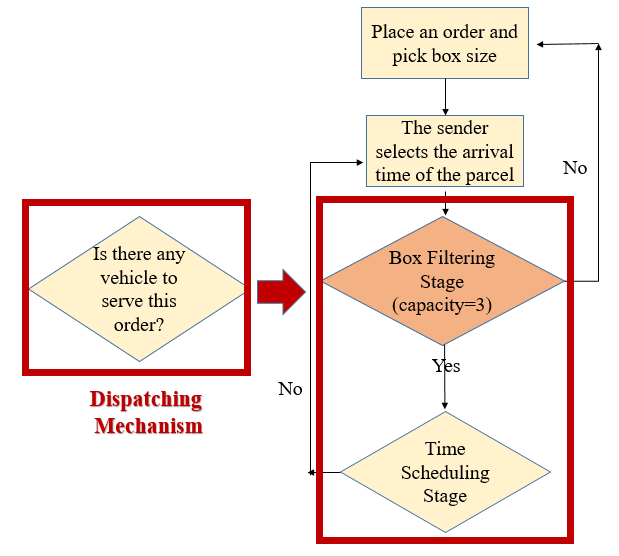
\includegraphics[width=1.0\textwidth]{./Thesis_figures/F6-1_dispatching_mechanism.PNG}
\caption{\large Dispatch mechanism consists of box filtering stage and simple time scheduling stage.}
\vspace{0.5cm}
\label{Fig:Dispatch_mechanism}
\end{figure}

\section{Box Filtering Stage }
When the sender’s delivery order is established, the system would generate a unique box index number of the order. Then, each digit of the box index has the different meaning. Take “221” as an example, the hundreds digit of the number means the id number of the vehicle, which delivers this parcel. Then, the tens digit of the number indicates the size of the box. The number of one means small size, the number of two means medium size, and the number of three indicates large size. The units digit of the number means the box location number, which ranges from zero to three. 
To sum up, in this case of box index number “221”, the number shows that the parcel is in the vehicle 2, which is placed in the medium box size, and the parcel is put into the first medium box.

\begin{figure}[H]
\centering
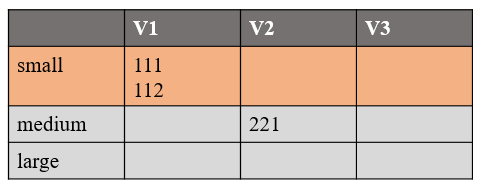
\includegraphics[width=0.85\textwidth]{./Thesis_figures/F6-2_caseOne_boxFiltering.PNG}
\caption{\large Case one of the car-box map.}
\vspace{0.5cm}
\label{Fig:CaseOne_carBox_Map}
\end{figure}

As illustrated in Figure 6.2, the figure shows the first case of the car-box map. In the figure, the top raw means different vehicles id, and the far left column means three kinds of box size. Then, the vehicle 1 has two box index number belonging to the \textbf{small box size}, the vehicle 2 has one box number belonging the medium box size, and the vehicle 3’s all boxes are empty.
As the delivery order with small box size is inserted to the system, the system will filter the suitable vehicles to the next stage according the form. Because the number of small box in vehicle 1 is two, the number of vehicle 2’s small boxes is zero, and the number of vehicle 3’s small box is zero as well. Each number of small box in each vehicle is lower than three. As a result, all three vehicles are the candidates which can enter the next stage.

\begin{figure}[t]
\centering
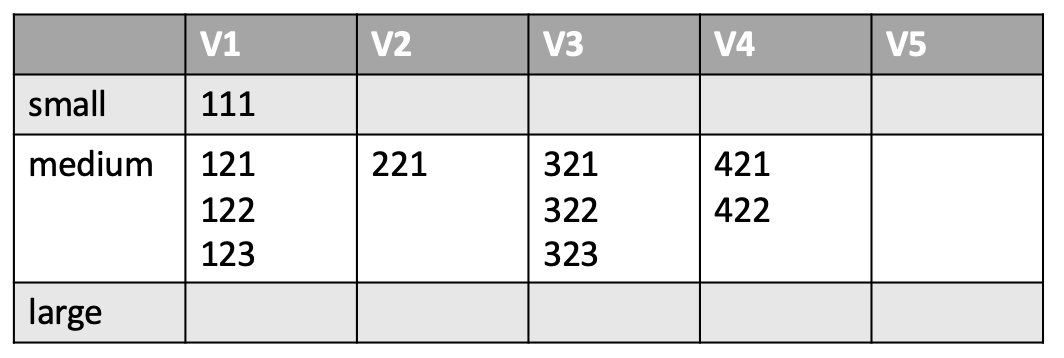
\includegraphics[width=0.85\textwidth]{./Thesis_figures/F6-3_caseTwo_boxFiltering.PNG}
\caption{\large Case two of the car-box map.}
\vspace{0.5cm}
\label{Fig:CaseTwo_carBox_Map}
\end{figure}

As illustrated in Figure 6.3, the form is the second case of the car-box map. As the system receives the delivery order with the medium box size, the box filtering execution starts. Therefore, vehicle 2, vehicle 4, and vehicle 5 are the candidates because all their occupancy of medium box are lower than three.

\section{Simple Time Scheduling Stage}

After passing the previous filtering stage, there are some vehicles entering into simple time scheduling stage. This stage aims to judge whether the new delivery request can be inserted into the delivery time schedule.

\begin{figure}[H]
\centering
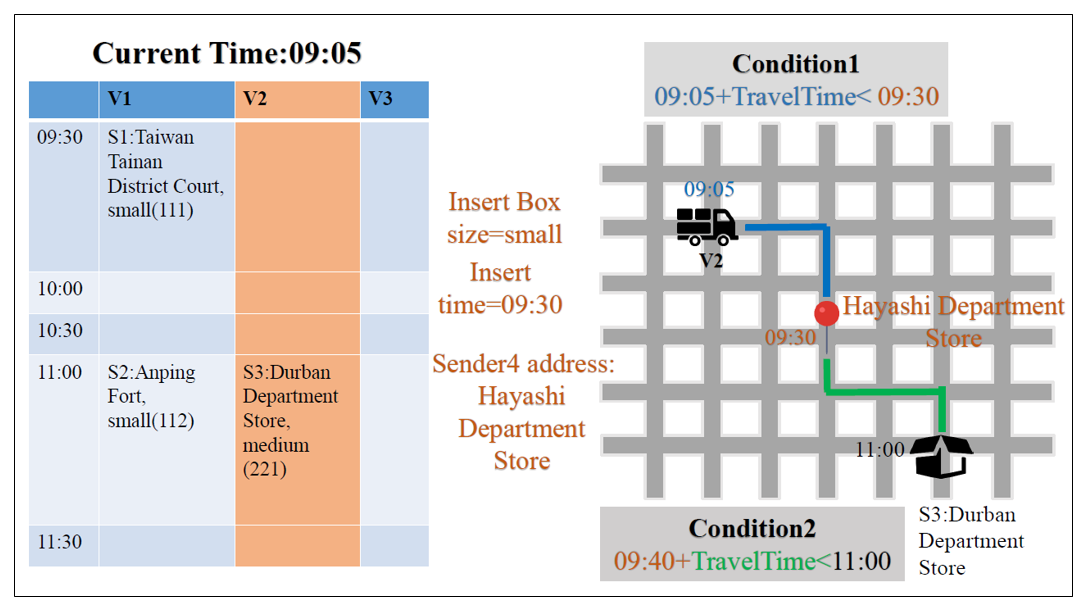
\includegraphics[width=1.14\textwidth]{./Thesis_figures/F6-4_caseOne_SchedulingStage.PNG}
\caption{\large Case one of simple time filtering stage.}
\vspace{0.5cm}
\label{Fig:CaseOne_TimeFiltering}
\end{figure}

As illustrated in Figure 6.4, this picture means the first case of simple time filtering stage.
In left side of the figure, the time schedule includes three vehicles with previous tasks, and the schedule starts from 09:30 AM to 11:30 AM. To be more specific, vehicle 1 has the delivery task of the sender 4 with the box index number “111”, which indicates the vehicle 1 has to arrive to the Taiwan Tainan District Court before 09:30 AM, and this task is located at the small box in the vehicle 1.
When the simulation time is 09:05 AM, the sender4 submits the delivery order request with the small box size and the expected arrival time to Hayashi Department Store is 09:30 AM.

Because the vehicle 1 has already the task of 09:30 AM, the system would turn to the next vehicle to deal with the request.
The right side of the figure shows the map with the vehicle 2’s routes which contains the new destination with the expected arrival time.
According to the map, the vehicle 2 has to meet two conditions. First condition is that after passing through the blue route, the vehicle 2 should arrive to Hayashi Department Store before 09:30 AM. 
When the vehicle 2 starts at 09:40 in Hayashi Department Store, and forwards to the Durban Department Store. Then, the second condition is that the vehicle 2 should arrive before 11:00 AM.
After satisfying the two above conditions, the sender 4’s delivery task would be inserted into the time schedule and come with the box index number. 

\begin{figure}[H]
\centering
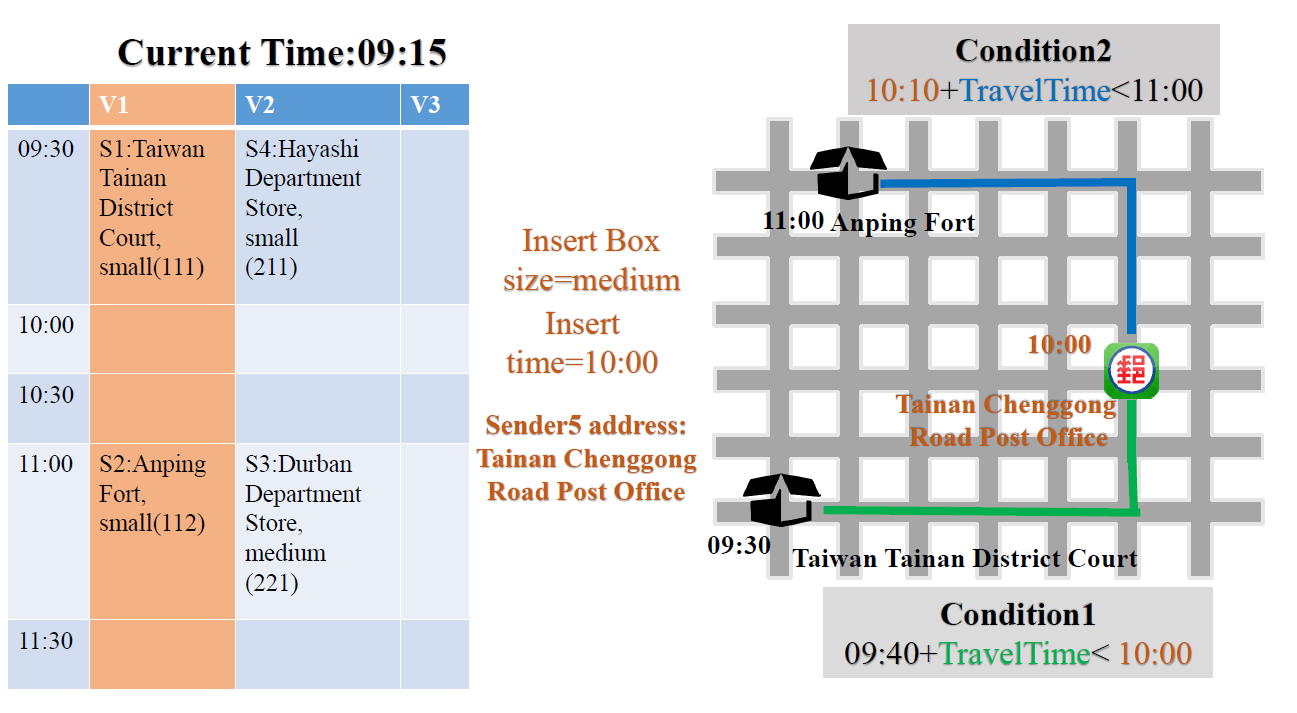
\includegraphics[width=1.14\textwidth]{./Thesis_figures/F6-5_caseTwo_SchedulingStage.PNG}
\caption{\large Case two of simple time filtering stage.}
\vspace{0.5cm}
\label{Fig:CaseTwo_TimeFiltering}
\end{figure}

As illustrated in Figure 6.5, this picture is the second case of simple time filtering stage. In left side of the figure, the time schedule includes three vehicles with four tasks. When the simulation time is 09:15 AM, the sender5 submits the delivery order request with the medium box size and the expected arrival time to Tainan Chenggong Road Post Office is 10:00 AM.
According to the box conditions of all vehicles, the system selects vehicle 1 to filter the sender 5’s delivery request. At the same time, the map in the right side of the figure show that this request has to meet the two conditions. Firstly, when the vehicle 1 arrives to the Taiwan Tainan District Court, the vehicle 1 would stop until 09:40, and would forward to Tainan Chenggong Road Post Office. The travel time of the green route should be less than twenty minutes. Secondly, after staying at Tainan Chenggong Road Post Office for ten minutes, the vehicle 1 will leave at 10:00 AM, and have to go to Anping Fort before 11:00 AM. 
As the vehicle 1 can fulfill the two conditions, the sender 5’s delivery request can be inserted into the time schedule.




\begin{figure}[H]
\centering
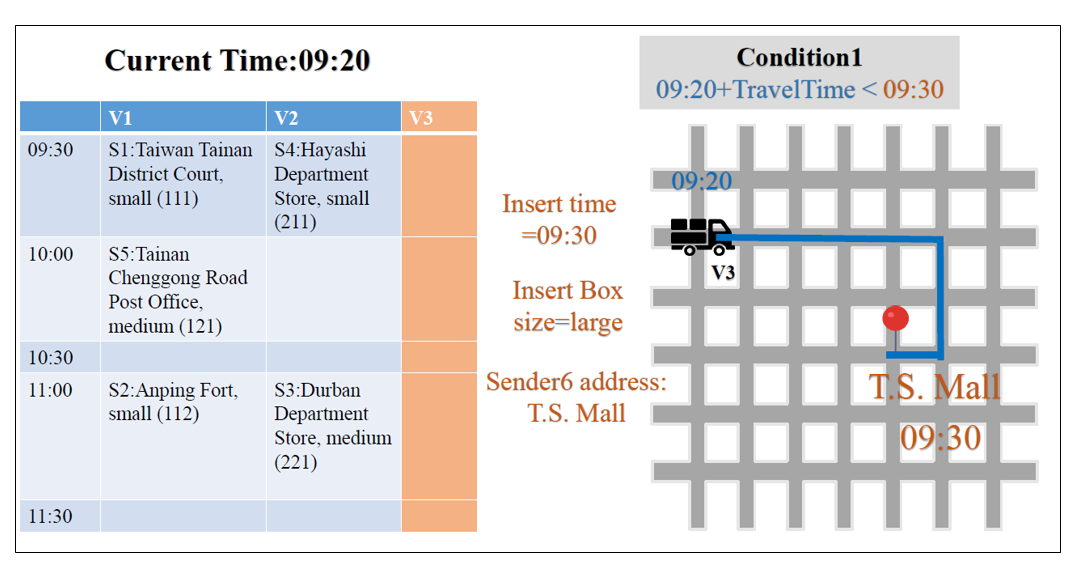
\includegraphics[width=1.14\textwidth]{./Thesis_figures/F6-6_caseThree_SchedulingStage.PNG}
\caption{\large Case three of simple time filtering stage.}
\vspace{0.5cm}
\label{Fig:CaseThree_TimeFiltering}
\end{figure}

As illustrated in Figure 6.6, this picture is the third case of simple time filtering stage. At simulation time of 09:20, the system receives the sender 6’s delivery request with the expected arrival time of 09:30 AM. Because the vehicle 1 and vehicle 2 already have the task of 09:30 AM, and the vehicle3 has to deal with this request. In right side of the figure, the vehicle 1 just has to match one condition because there is no task before this request. Thus, when the vehicle3 starts from current position at 09:20, the travel time of blue route to T.S. Mall has to be less than ten minutes.
Moreover, the vehicle will execute the tasks according to the time schedule, and follow the flow chart of delivery process mentioned in the Figure 5.1 and Figure 5.2.


\section{User Scenario}

This section shows the user scenarios when the vehicle arrives to the destination. The scenarios includes the sender's scenario and the receiver's scenario.

\subsection{Sender Scenario}

\begin{figure}[H]
\centering
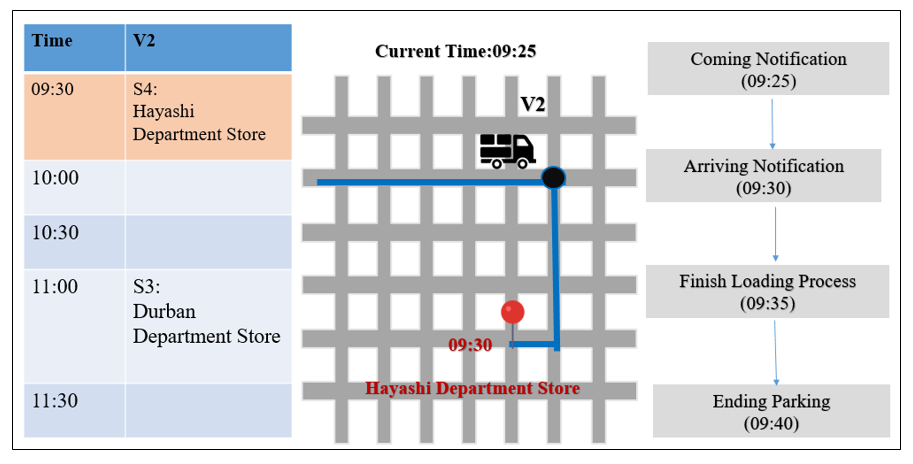
\includegraphics[width=1.14\textwidth]{./Thesis_figures/F6-7_senderScenario.PNG}
\caption{\large The sender's scenario of parcel delivery process.}
\vspace{0.5cm}
\label{Fig:senderScenario_DeliveryPorcess}
\end{figure}

As illustrated in Figure 6.7, the vehicle 2 would demonstrate how to react in the task of 09:30 AM in the sender scenario of delivery process. As the simulation time is 09:25, the vehicle 2 would be at the black point of position, and the SUMO server would use FCM to send coming notification to the sender4. Then, when the simulation time is 09:30 AM, the vehicle 2 would be at Hayashi department store, start to park for ten minutes, and the sender4 would get the arriving notification.
As the simulation time is 09:35, the vehicle 2 will finish the loading process of the parcel. Finally, at the simulation of 09:40, the vehicle 2 would end parking in the Hayashi department store, and would forward to the next station.

\subsection{Receiver Scenario}

\begin{figure}[H]
\centering
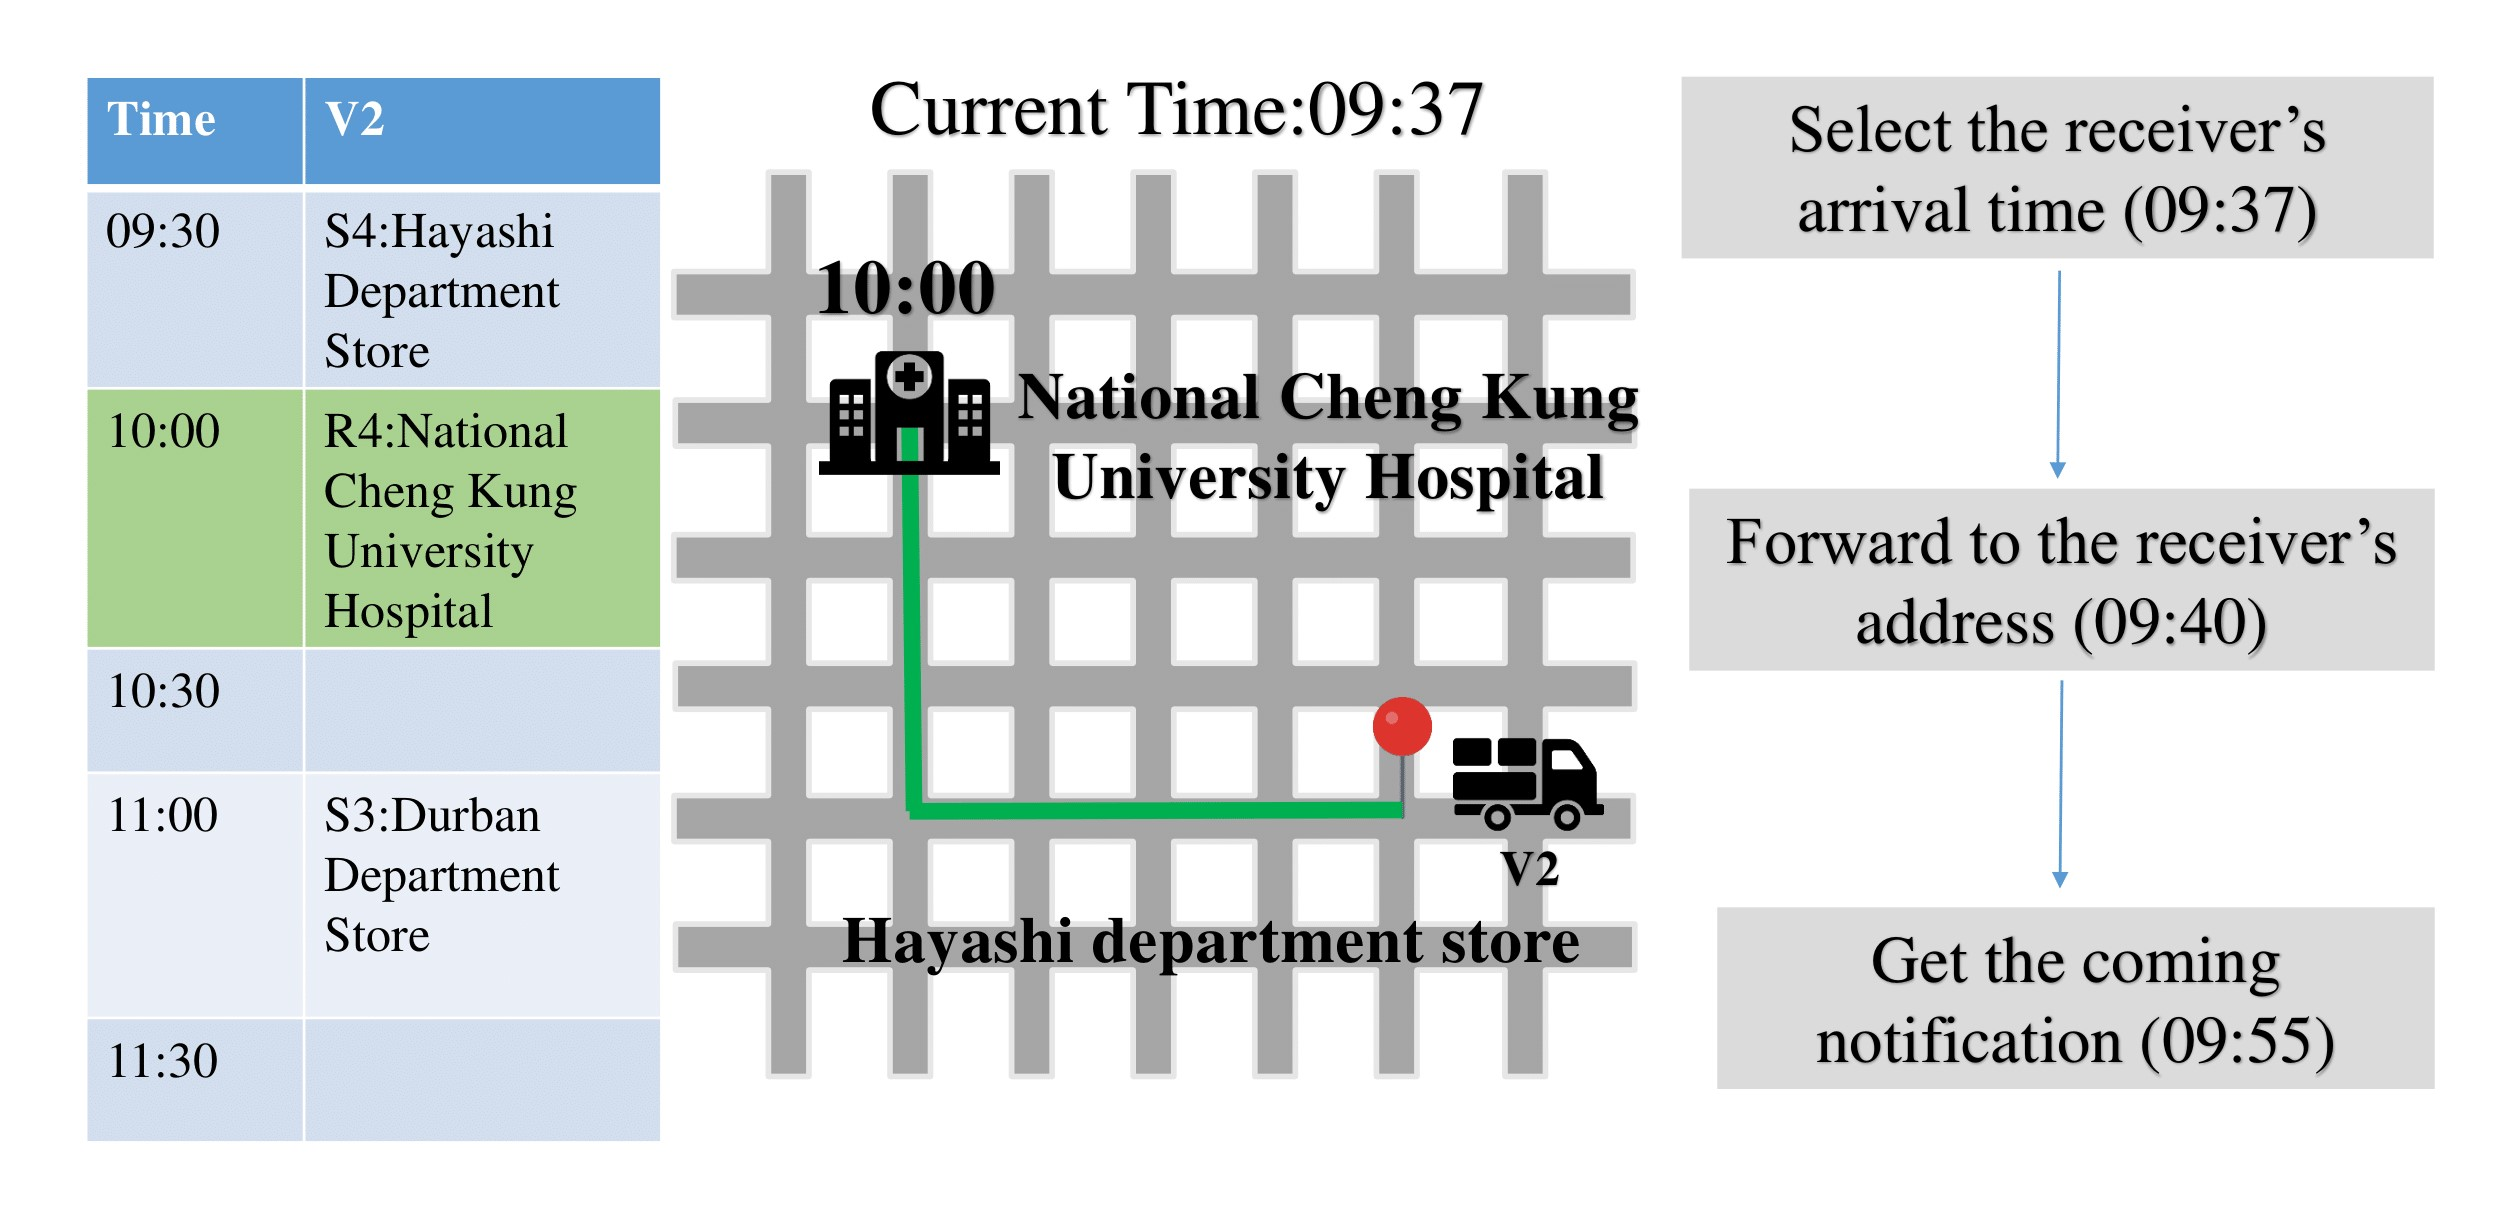
\includegraphics[width=1.14\textwidth]{./Thesis_figures/F6-8_receiverScenario1.PNG}
\caption{\large The receiver's first scenario of parcel delivery process.}
\vspace{0.5cm}
\label{Fig:FirsrtReceiverScenario_deliveryProcess}
\end{figure}

As illustrated in Figure 6.8, the vehicle 2 would demonstrate how the receiver 4 participates in the delivery process. Firstly, the vehicle 2 follows the sender scenario in figure 6.6, and the vehicle2 has already finished the loading process.
However, the current simulation time is 09:37 AM, and the vehicle 2 starts to deal with the receiver 4’s task of National Cheng Kung University Hospital (NCKUH). When the simulation time is 09:40, the vehicle 2 leaves Hayashi department store, and forwards to NCKUH. Besides, As the time is 09:55 AM, the vehicle 2 would be close to the NCKUH, and the receiver 4 would get the coming notification.


\begin{figure}[H]
\centering
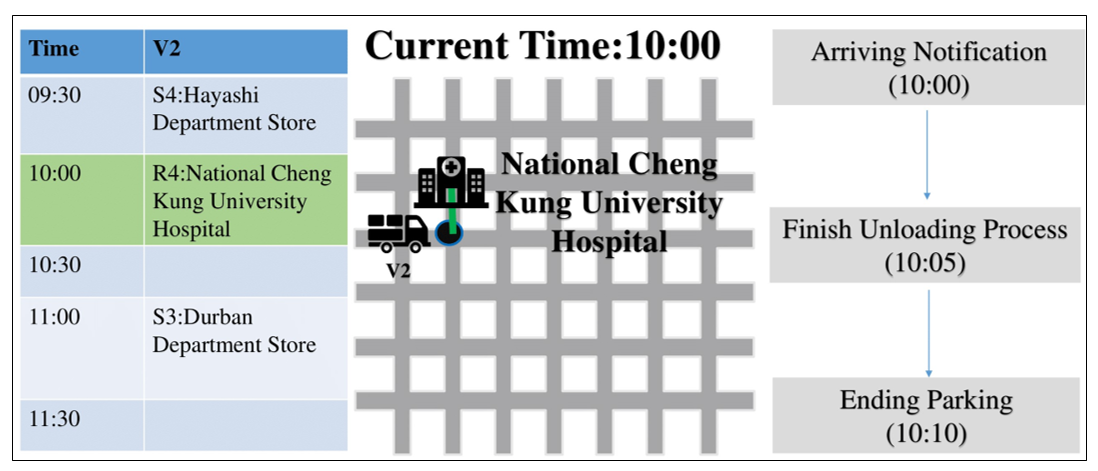
\includegraphics[width=1.14\textwidth]{./Thesis_figures/F6-9_receiverScenario2.PNG}
\caption{\large The receiver's second scenario of parcel delivery process.}
\vspace{0.5cm}
\label{Fig:Second_ReceiverScenario_DeliveryProcess}
\end{figure}

As illustrated in Figure 6.9, the vehicle 2 will show the receiver’s scenario of delivery process. As the simulation is 10:00 AM, the receiver 4 would get the arriving notification, and prepare to pick up the parcel. At the time of 10:05 AM, the vehicle 2 would finish the unloading process. Finally, the vehicle 2 would end parking in National Cheng Kung University Hospital (NCKUH), and forward to the next station.





%------------------------- Simulation -------------------------%



\chapter{Simulation}\label{Chap:Simulation}
%------------------------- Simulation -------------------------%

\section{Simulation Setting}

\subsection{Simulator}
SUMO is used to be the simulator for running the parcel delivery simulation [12]. “Simulation of Urban Mobility”, or “SUMO” for short, is an open source, multi-modal traffic, highly portable, microscopic and continuous road traffic simulator. The method to control the SUMO simulator is to use the TraCI client Python Application Program Interface (API), which is available in SUMO packages.

\subsection{Road Network}

The dataset, which was acquired from OpenStreetMap \cite{Haklay2008} , uses the road network of part of Tainan, which is the south of Taiwan. The region of the selected road contains the partial Tainan East District, Tainan West Central District, partial Tainan North District, partial Tainan South District, and partial Tainan Anping District.

The road network, which is pruned by estimating unreachable streets and roads for a truck, contains 25069 roads segments, and 6785 junctions with approximately $50km^{2}$ in the downtown of Tainan.

\begin{figure}[H]
\centering
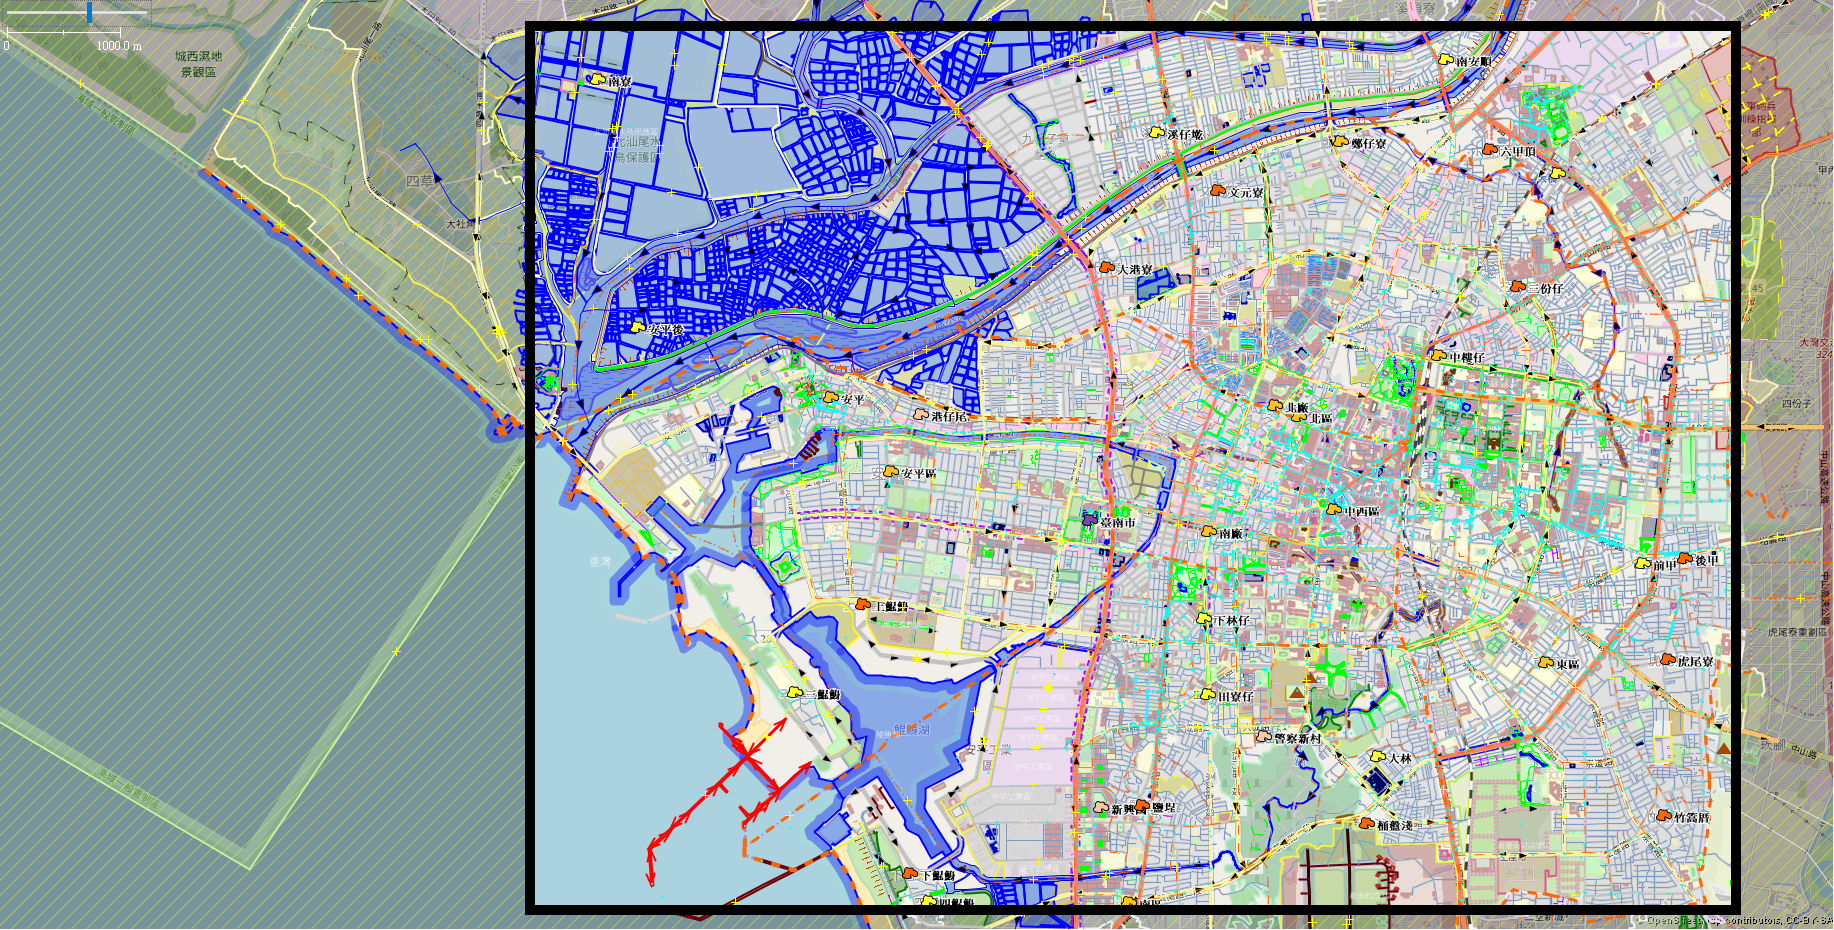
\includegraphics[width=1.0\textwidth]{./Thesis_figures/F7-1_Openstreetmap.PNG}
\caption{\large Downtown area of Tainan in OpenStreetMap.}
\vspace{0.5cm}
\label{Fig:DowntownArea_in_OpenStreetMap.}
\end{figure}


\begin{itemize}
\item
Figure 7.1 shows the road network on OpenStreetMap.

\item
Figure 7.2 illustrates the road network of truck passable segments on SUMO Map.

\item
Figure 7.3 shows the selected road network on Google Map.

\end{itemize}

\begin{figure}[H]
\centering
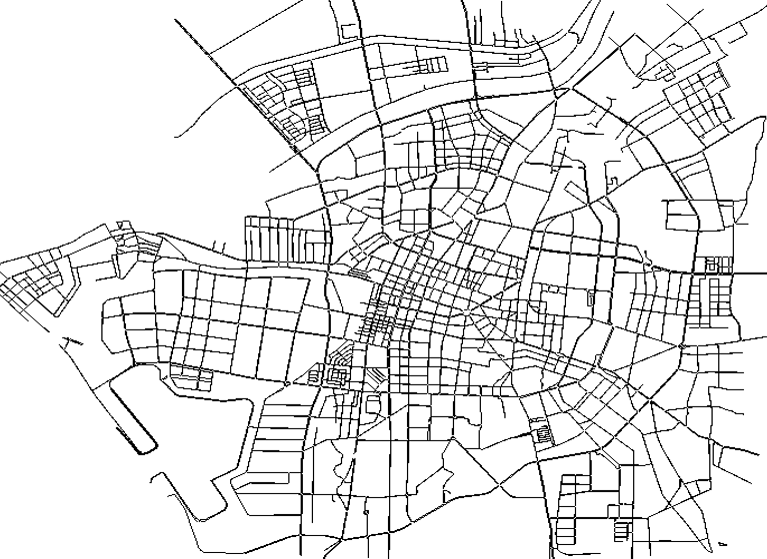
\includegraphics[width=1.0\textwidth]{./Thesis_figures/F7-2_SUMOMap.PNG}
\caption{\large  Service region of the experiment on SUMO.}
\vspace{0.5cm}
\label{Fig:SUMOMap}
\end{figure}

\begin{figure}[H]
\centering
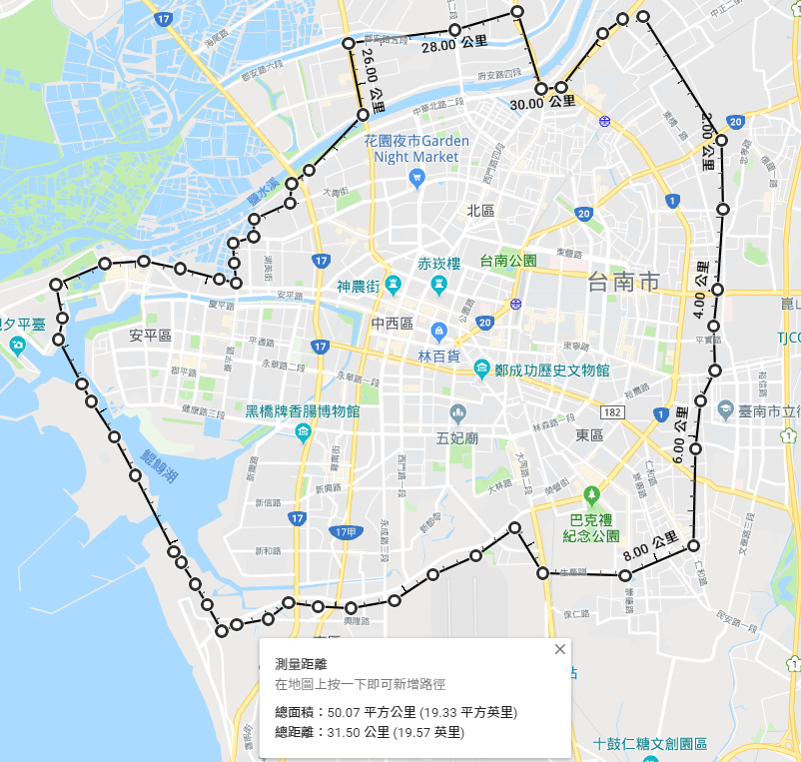
\includegraphics[width=1.0\textwidth]{./Thesis_figures/F7-3_GoogleMap.PNG}
\caption{\large Service region of the experiment on Google Map.}
\vspace{0.5cm}
\label{Fig:GoogleMap}
\end{figure}

\subsection{Parameters}
Parameters of the simulation are showed in Table 7.1. Note that the number of trucks is three from the simulation time $T_{start}$ to $T_{end}$. 
Then, the maximum speed of truck is 18 km/hr, and the range of speed limit on each lane is 10-100 km/hr. It is noteworthy that trucks will not exceed the speed limit on each lane even the truck has a higher maximum speed. Besides, a truck has nine boxes which are grouped by small size, medium size, and large size. The capacity of each box size is three. Then, the loading process time is five minutes, and the unloading process time is five minutes as well. Finally, when the SUMO server counts the travel time of the vehicle, which is equal to the driving distance divided by the estimated average vehicle speed. Thus, the estimated average vehicle speed is 14.4 km/hr.

\begin{figure}[H]
\centering
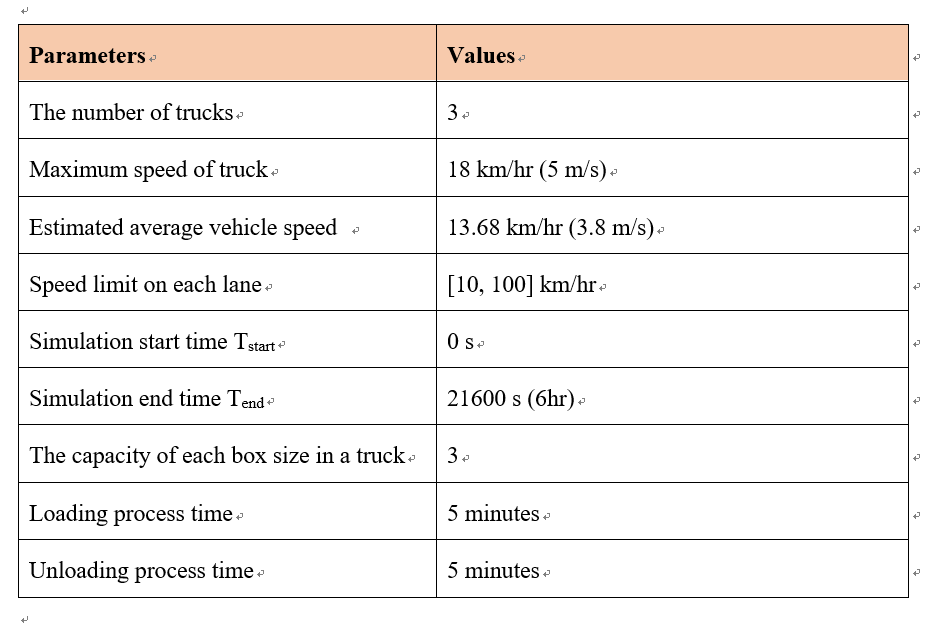
\includegraphics[width=1.0\textwidth]{./Thesis_figures/F7-4_parameters.PNG}
\caption{\large Parameters of simulation.}
\vspace{0.5cm}
\label{Fig:Parameters_of_Simulation}
\end{figure}

\subsection{Average Vehicle Speed Estimation}

As illustrated in Figure 7.5, the horizontal axis represents the different routes in Tainan downtown, and the vertical axis shows the vehicle's speed. Take the route 1 as an example, the route1 starts from Anping Fort to the Taiwan Tainan District Court, and the driving distance is 2.9 kilometers. In this case, the blue line represents the maximum speed of truck in SUMO, and the green line indicates the average vehicle speed in Google Map, and the orange line is real average vehicle speed in SUMO. Thus, according to the seven cases in this figure, to avoid the delay in delivery, the study sets estimated average vehicle speed to \textbf{"3.80"} m/s (13.68 km/hr).


\begin{figure}[H]
\centering
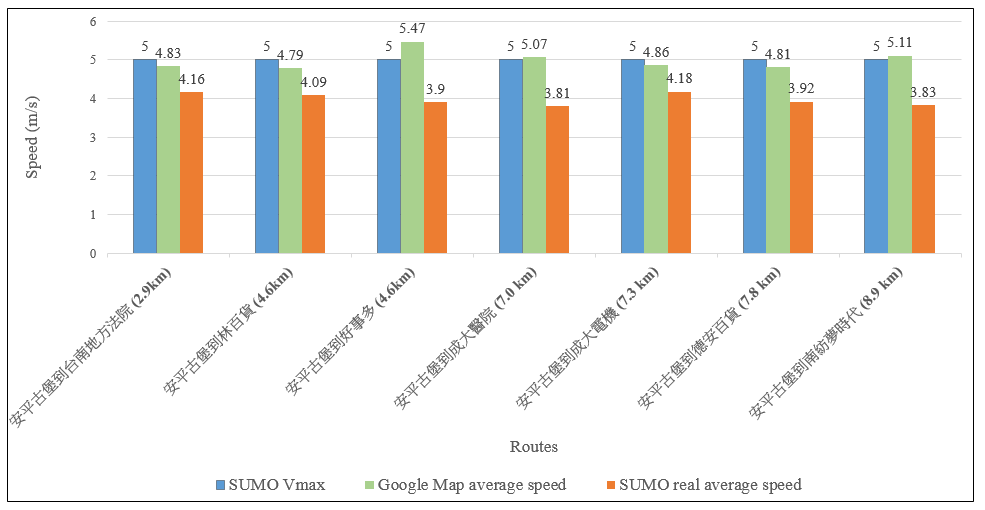
\includegraphics[width=1.14\textwidth]{./Thesis_figures/F7-5_speedEstimation.PNG}
\caption{\large Average vehicle speed estimation.}
\vspace{0.5cm}
\label{Fig:Average_vehicleSpeedEstimation}
\end{figure}

\section{Simulation Result}
It this section, there are five stages of simulation results, which includes simulation initialization, the sender’s request insertion, the loading process, the receiver’s request, and the unloading process.

As illustrated in Figure 7.6, the picture shows the simulation initialization without any request insertion. According to the time schedule in the left side of the Figure, each vehicle has different column color, which indicates the distinct routes. Take the vehicle 2 as an example, the system arranges blue route with one task in the right side of the Figure. Thus, the vehicle 2 would arrive to the Durban Department Store before 11:00 AM, and stay in the destination until 11:10 AM.

\begin{figure}[H]
\centering
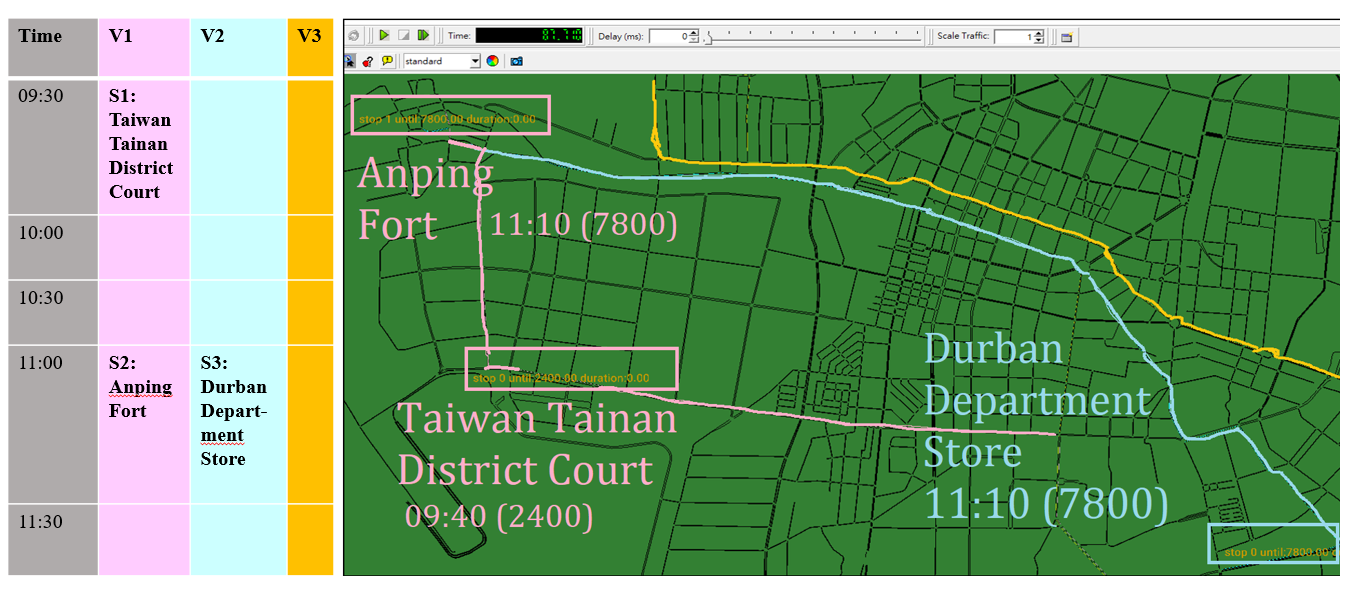
\includegraphics[width=1.12\textwidth]{./Thesis_figures/F7-6_initialization.PNG}
\caption{\large Initialization of Simulation.}
\vspace{0.5cm}
\label{Fig:Initialization_of_Simulation}
\end{figure}

As illustrated in Figure 7.7, the figure shows how the original route changes after receiving the sender’s request.
The left side of graph shows that when the simulation time is 1203 seconds, which means 09:20:03, and the user wants to pick 09:30 as the expected sender’s arrival time. Then, the vehicle 2 follows the yellow route. However, at the time of 1218 seconds, which means 09:20:18, the vehicle 2 replaces original blue route with yellow route and would stop at Hayashi Department Store until 09:40 AM.

\begin{figure}[H]
\centering
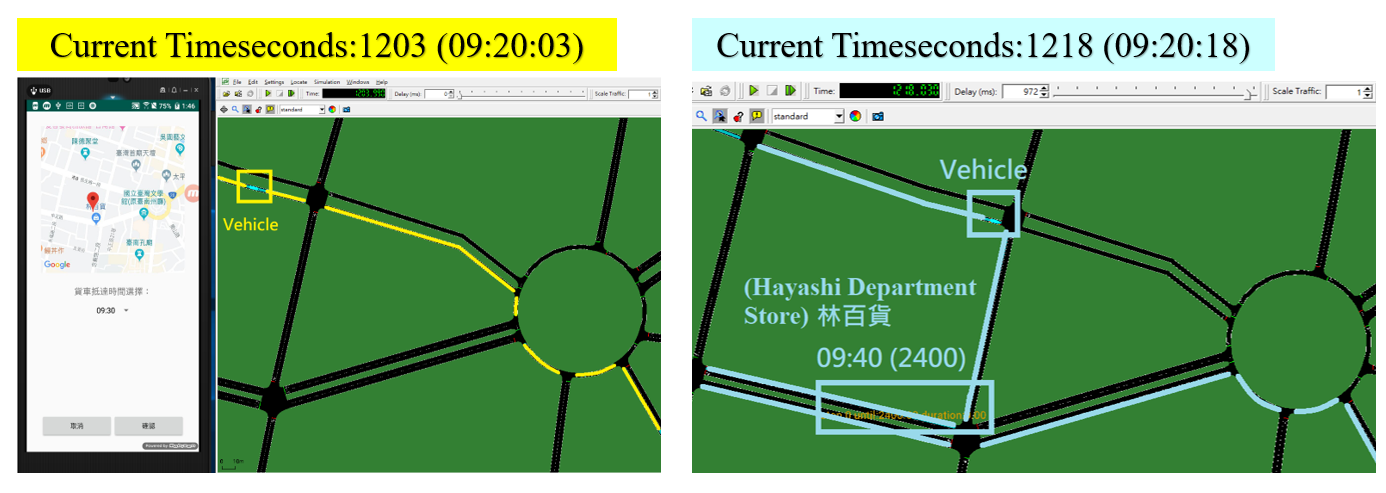
\includegraphics[width=1.12\textwidth]{./Thesis_figures/F7-7_senderRequest.PNG}
\caption{\large The Sender’s Request Insertion in simulation.}
\vspace{0.5cm}
\label{Fig:sender_request}
\end{figure}


As illustrated in Figure 7.8, the receiver’s phone in the left side of the figure gets the notification of finishing loading process at sender’s address in 09:35. The box index number “211” has the value of one, which means that the parcel exists in the vehicle 2. Thus, the receiver can start to select the expected arrival time of the parcel.

\begin{figure}[H]
\centering
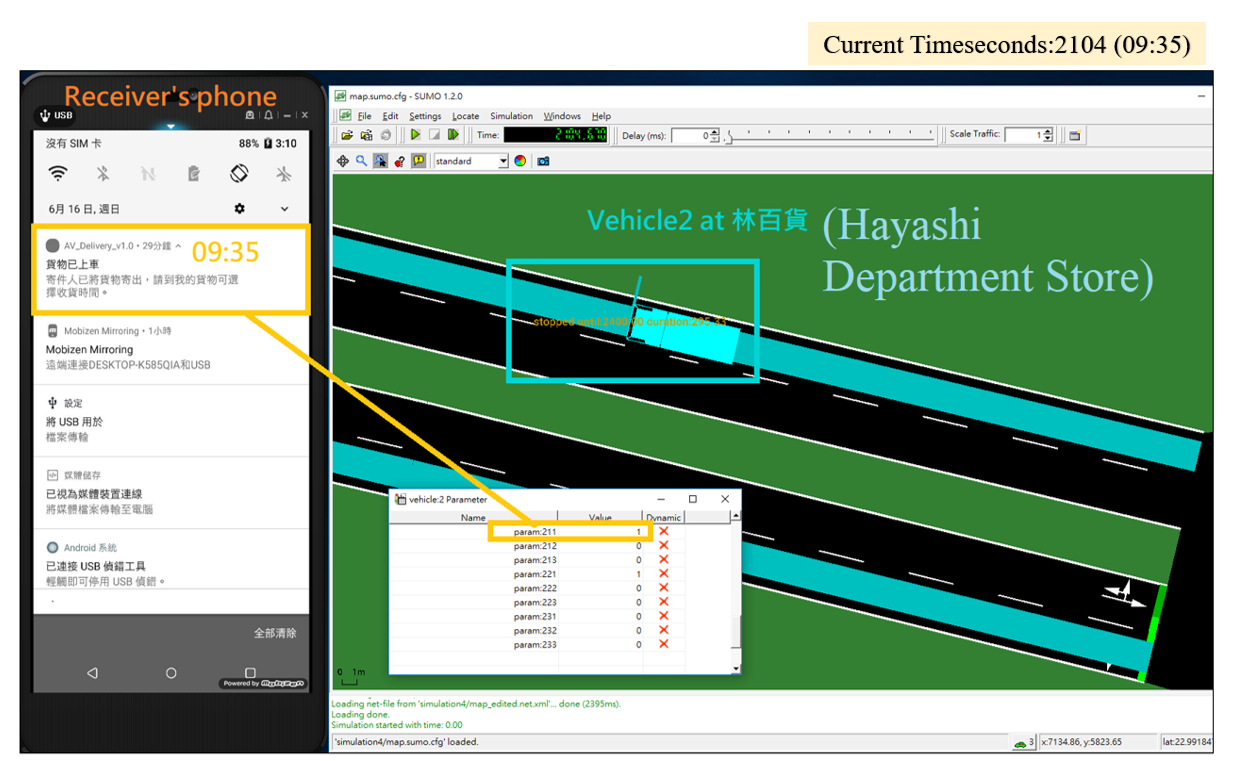
\includegraphics[width=1.12\textwidth]{./Thesis_figures/F7-8_loadingProcess.PNG}
\caption{\large The loading process at the sender’s sddress in simulation.}
\vspace{0.5cm}
\label{Fig:LoadingProcess}
\end{figure}


As illustrated in Figure 7.9, the left side of the figure shows that at the simulation time of 2104 seconds, which means 09:35:04, the receiver selects 10:00 AM as the arrival time. 
Moreover, at 09:36:16, the vehicle 2 replaces the original blue route with the yellow route after inserting the receiver’s request. This route in right side of the figure shows that the vehicle 2 would stop at the entrance of Kuang-Fu campus in National Cheng Kung University in 10:00.

\begin{figure}[H]
\centering
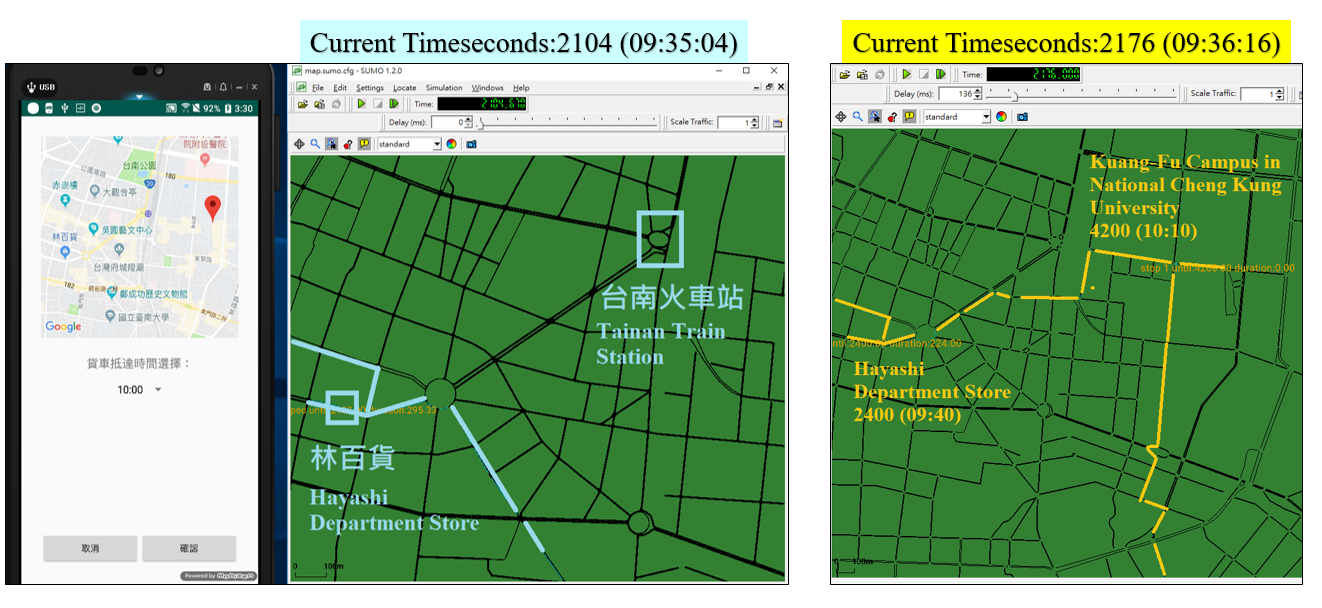
\includegraphics[width=1.12\textwidth]{./Thesis_figures/F7-9_receiverRequest.PNG}
\caption{\large The receiver’s request insertion in simulation.}
\vspace{0.5cm}

\label{Fig:Receiver_request}
\end{figure}

As illustrated in Figure 7.10, the receiver receives the arriving notification of the parcel at 10:00 AM. Then, at 10:07:29, the vehicle 2 finishes the unloading process and the parameters of box also changes. Besides, the vehicle 2 still has to stay in receiver’s address until 10:10 AM.

\begin{figure}[H]
\centering
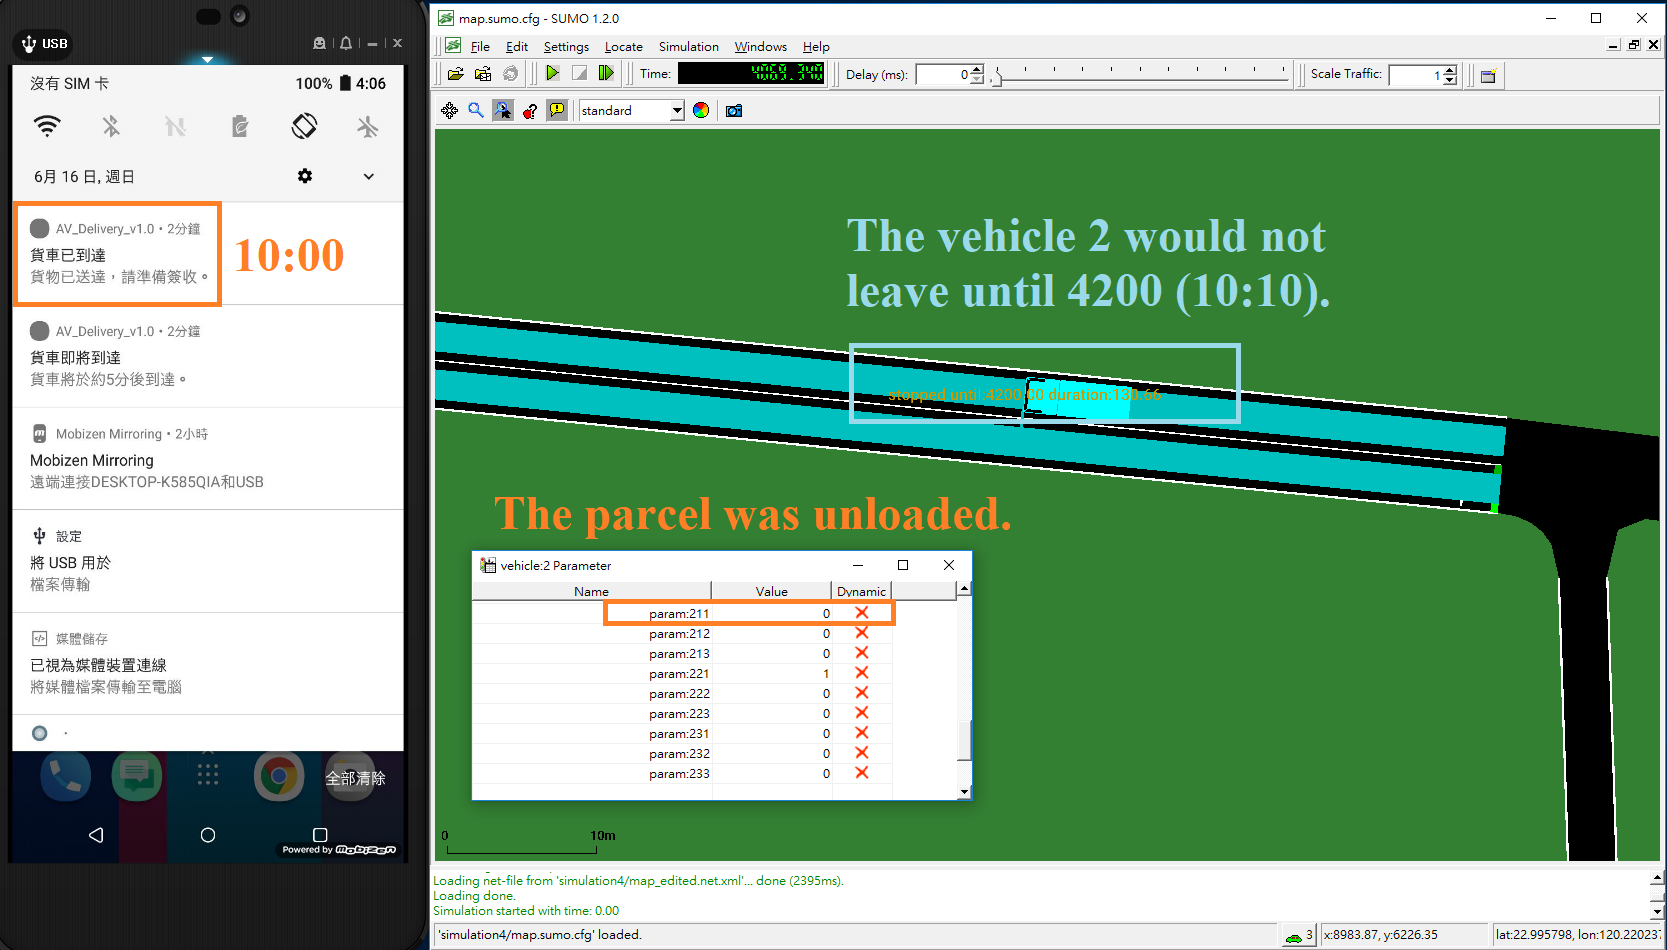
\includegraphics[width=1.12\textwidth]{./Thesis_figures/F7-10_unloadingProcess.PNG}
\caption{\large The unloading process at the receiver’s address in simulation.}
\vspace{0.5cm}
\label{Fig:unloading_request}
\end{figure}









%%%%%%%%%%%%%%%%%%%%%%%%%%%%%%%%%%%%%%%%%%%%%%%%%%%%%%%%%%%%%%%%%%%%%%%




\chapter{Conclusion and Future Work} \label{Chap:Conclusion}
%------------------------- Conclusion -------------------------%

\section{Conclusion}
The thesis implemented a vehicle dispatching and monitoring system to simulate the parcel delivery process. In this system, the thesis used the commands of Traffic Control Interface (TraCI) to manipulate vehicle’s behavior, and retrieve the vehicle’s values in SUMO simulator. As the system received the delivery order request from Android client, the system would use dispatching mechanism to judge whether this order can be established successfully or not. If there is no vehicle that can serve this request, the user would pick their box size or select the other arrival time of the package, and submit the order again. In contrast, as the order is established, the system would arrange the routes via the time schedule and change the container’s value. With this schedule, the system can deal with the delivery order request more orderly. 

Besides, the system would set the parking duration to simulate the loading and unloading process when the vehicle arrives to the destination. As a result, the users can have enough time to interact with the truck in simulator. 

Finally, the thesis used three trucks and nine containers to simulate the delivery process including sender’s scenario and receiver’s scenario in the downtown area of Tainan. By using the vehicle dispatching and monitoring system, the administrator can arrange the route dynamically and track the vehicle’s movement immediately, and monitor the simulation of the parcel delivery process.




\section{Future Work}

There are some issues that should be discussed to complete the vehicle dispatching and monitoring system.

\begin{itemize}


\item
\textbf{Scalability}: So far the system only contains three trucks in the downtown area of Tainan, whose area is $50km^{2}$. Thus, in the future the system would be used in larger map and distribute more trucks into different areas according to the quantity of parcels. Besides, In the dispatch mechanism, the system current empirical time scheduling method to filter the suitable order. However, in the future the system should have the ability to implement different routing algorithms to schedule tasks on the same simulation platform.

\item
\textbf{Quantity}: Now the system runs the delivery simulation with a small amount of order requests. However, the system has to deal with a batch of orders in a brief period of time in the future.

\item
\textbf{Accuracy}: When it comes to scheduling the task, the system has to calculate the travel time of the new route. Thus, the accuracy of the estimated vehicle speed is very crucial and this value should be actually measured by the real-time road conditions.

\end{itemize}

\cite{Fischer}
\cite{Jiang2018}


} \end{thesis}

%------------------------- References -------------------------%
\singlespace {\large

\bibliography{Reference-Yen}

}

\bibliographystyle{IEEEtran}

\doublespace

\begin{vita}
%------------------------- Vita -------------------------%
\Thesisspace \large{

Kang Yen was born on December 3, 1993, in Yunlin, Taiwan.  He received the B.S. degree in Electrical Engineering from National Cheng Kung University, Taiwan, in 2017. In September 2017, he enrolled at the National Cheng Kung University as a master student in the Institute of Computer and Communication Engineering.

}\end{vita}

\end{document}

